\documentclass[preprint]{iacrtrans}

\usepackage{paper}

\title{An exploration of ISEs for AES on RISC-V}
\keywords{AES, ISE, RISC-V}

\ifbool{anonymous}{%
\author{}
\institute{}
}{%
\author{
Ben Marshall\inst{1}                \and
Dan Page\inst{1}                    \and
Markku-Juhani O. Saarinen\inst{2}   \and
(Andy/ Richard / Barry / Claire?)
}
\institute{
    Department of Computer Science, University of Bristol \\ \email{{ben.marshall,daniel.page}@bristol.ac.uk}
    \and
    PQShield, Oxford \\ \email{mjos@pqshield.com}
}
}%

\begin{document}

% =============================================================================

\maketitle

\begin{abstract}
Secure, efficient execution of AES represents an imperative, and therefore 
well studied requirement in many use-cases.  Use of an
Instruction Set Extension (ISE)
is one approach to addressing this requirement, and, as a result, ISEs for 
AES exist in many ISAs.  
However, RISC-V is a (relatively) new ISA that lacks such an ISE: this gap
motivates our work.  In specific terms, and set against on-going effort to 
standardise cryptographic ISEs for RISC-V, we
1) survey the state-of-the-art wrt. ISEs for AES,
2) implement and evaluate five different ISEs for AES,
   one of which is novel,
3) explore how the B 
   (or bit manipulation) 
   extension
   to RISC-V can be harnessed for efficient implementation of AES-GCM,
   and
4) demonstrate how an ISE for AES can hardened against DPA-style attacks.
\end{abstract}

% =============================================================================

\section{Introduction}
\label{sec:intro}
% =============================================================================

\paragraph{Implementing the Advanced Encryption Standard (AES).}

%
% Commented out since CHES folks know the histories.
%
%In October $2000$, NIST pronounced Rijndael~\cite{DaeRij:98,DaeRij:02}, 
%a design due to Daemen and Rijmen, 
%as winner of a $5$-year standardisation process~\cite{NBBBDFR:01} instigated 
%to identify a replacement for the incumbent
%Data     Encryption Standard (DES)~\cite{FIPS:46} 
%block cipher; the resulting 
%Advanced Encryption Standard (AES)~\cite{FIPS:197} 
%was announced in $2001$.

Compared to more general workloads, cryptographic algorithms like AES
present a significant implementation challenge.
They involve computationally intensive and specialist functionality,
are used in a wide range of contexts
and
form a central target in a complex attack surface.
The demand for efficiency is a clear example in two ways.
First,
cryptography often represents an enabling technology vs. a feature and
is often viewed as an overhead from a user's perspective.
Addressing this is
complicated by constraints associated with the context, e.g., a demand 
for
high-volume, 
 low-latency, 
high-throughput, 
 low-footprint, 
and/or 
 low-power
 implementations.
Second,
although efficiency is a goal in itself, it {\em also} 
acts as an enabler for security.
This is because one {\em should not}
compromise security to meet efficiency requirements.
Hence a more efficient implementation leaves greater margin to deliver
countermeasures against attack.

AES is an interesting casestudy wrt. secure, efficient implementation.
For example,
per the request for candidates announcement,\footnote{%
\url{https://www.govinfo.gov/content/pkg/FR-1997-09-12/pdf/97-24214.pdf}
} the AES process was instrumental in popularising a model in which
{\em both}
``security''
(e.g., resilience against cryptanalytic attack)
{\em and}
``algorithm and implementation characteristics''
form important quality metrics for the {\em design}, in order to facilitate
techniques for higher quality {\em implementations} of it.
Additionally,
the design {\em and} implementations of AES are long-lived.
The importance of AES has led to special emphasis on related
research and development effort before, during, and, most significantly, 
after the AES process.
The $20+$ years since standardisation have forced an evolution of 
implementation techniques, to match changes in the technology 
and attack landscape.  For example,~\cite[Section 3.6]{NBBBDFR:01} covers
implementation (e.g., side-channel) attacks: this field has become richer,
and the associated threat more dangerous during said period.

% -----------------------------------------------------------------------------

\paragraph{Support via Instruction Set Extensions (ISEs).}

A large space of implementation styles often exist
for a given cryptographic algorithm.
Techniques can be
   algorithm-agnostic
   or
   algorithm-specific,
and based on the use of   
   hardware              only,
                software only,
   or
   a hybrid approach using ISEs ~\cite{GalBer:11,BarGioMar:09,RegIen:16}.
For the ISE case, the aim is to identify through benchmarking, pieces of
algorithm-specific functionality which are inefficiently represented in the
base ISA.
Said functions are then implemented in hardware, and exposed to the
programmer via one or more new instructions.

ISEs are an effective option for {\em both}
high-end, performance-oriented
and
 low-end, constrained
platforms. 
They are particularly effective for the latter where resource constraints
are tightest.
An ISE can be smaller and faster than a pure software implementation,
and more efficient in terms of performance gain per additional logic gate
than a hardware-only option.

Abstractly, an ISE design constitutes
an {\em interface} to domain-specific functionality through the
addition of instructions to a base ISA.
As a fundamental and long-lived computer systems interface, the design
and extension of an ISA demands careful consideration
(cf.~\cite[Section 4]{Gueron:09}). 
and the production of a concrete ISE design is not trivial.
It must deliver a quantified improvement to the workload in 
question (however measured) {\em and}
consider numerous design goals including but not limited to:

\begin{itemize}
\item Limiting the number and complexity of changes and interactions with the
    parent ISA.
\item Avoiding the addition of too many instructions, or requiring large
    additional hardware modules to implement. This will hurt commercial
    adoption of the ISA.
\item Adhering to the design constraints and philosophies of the base ISA.
\item Maximising the utility of the additional functionality,
      i.e.,
      favour general-purpose over special-purpose functionality.
      Special-purpose functions can be justified in terms of how frequently
      the workload is required.
      For example, though an AES ISE might {\em only}
      be useful for AES, a webserver might execute AES millions of times
      per day.
\end{itemize}

\noindent
The x86 architecture provides many examples of ISE design,
having been extended numerous times by Intel and AMD.
Various generations of
non-cryptographic
Multi-Media      eXtensions (MMX),
Streaming SIMD  Extensions (SSE),
and
Advanced Vector Extensions (AVX)
support numerical algorithms via vector (or SIMD) vs. scalar computation.  
Likewise, the
    cryptographic
Advanced Encryption Standard New Instructions (AES-NI)~\cite{Gueron:09,DruGueKra:19}
ISE
supports AES: it significantly improves latency and throughput
(see, e.g.,~\cite{FazLopOli:18}),
and represents a useful casestudy in the design goals above:
it adds just $6$ additional (vs. $1500+$ total) instructions,
reduces overhead by sharing the pre-existing XMM register file,
and facilitates compatibility via the
\VERB{CPUID}~\cite[Chapter 20]{X86:1:18}
feature identification mechanism.
It is also (sometimes un-expectedly) useful beyond AES:
the Gr{\o}stl hash function ~\cite{GKMMRST:11} uses the S-box,
and
the YAES~\cite{BosVer:14} authenticated encryption scheme uses a full round.
It can even be used to accelerate the Chinese SM4 block cipher.\footnote{\url{https://github.com/mjosaarinen/sm4ni}}

% =============================================================================


% =============================================================================

\section{Background}
\label{sec:bg}

% -----------------------------------------------------------------------------

\subsection{AES  specification}
\label{sec:bg:aes_spec}
% =============================================================================

% -----------------------------------------------------------------------------

\paragraph{Syntax.}

As a block cipher, AES defines two algorithms
\[
\begin{array}{lcl}
\ALG{Enc} &:& \SET{ 0, 1 }^{8 \cdot 4 \cdot Nk} \times \SET{ 0, 1 }^{8 \cdot 4 \cdot Nb} \rightarrow \SET{ 0, 1 }^{8 \cdot 4 \cdot Nb} \\
\ALG{Dec} &:& \SET{ 0, 1 }^{8 \cdot 4 \cdot Nk} \times \SET{ 0, 1 }^{8 \cdot 4 \cdot Nb} \rightarrow \SET{ 0, 1 }^{8 \cdot 4 \cdot Nb} \\
\end{array}
\]
st.
$
m = \ALG{Dec}( k, c = \ALG{Enc}( k, m ) ) .
$
That is, given a plaintext $m$ and cipher key $k$, \ALG{Enc} encrypts $m$ 
under $k$; given the same $k$, \ALG{Dec} will invert \ALG{Enc} and so the
{\em same} $m$ can be recovered from the associated ciphertext $c$.  
In addition, it defines an algorithm
\ALG{KeyExp}
that expands~\cite[Section 5.2]{FIPS:197} the cipher key into a sequence 
of round keys then used by
\ALG{Enc}
or
\ALG{Dec};
where appropriate, we use
\[
\begin{array}{lcl}
\ALG{Enc-KeyExp} &:& \SET{ 0, 1 }^{8 \cdot 4 \cdot Nk} \rightarrow \SET{ 0, 1 }^{( 8 \cdot 4 \cdot Nb ) \times ( Nr + 1 )} \\
\ALG{Dec-KeyExp} &:& \SET{ 0, 1 }^{8 \cdot 4 \cdot Nk} \rightarrow \SET{ 0, 1 }^{( 8 \cdot 4 \cdot Nb ) \times ( Nr + 1 )} \\
\end{array}
\]
to denote said algorithm as specialised to suit
\ALG{Enc}
and
\ALG{Dec}
respectively.

% -----------------------------------------------------------------------------

\paragraph{Parameterisation.}

An AES parameter set~\cite[Figure 4]{FIPS:197}
is a triple
$
\TUPLE{ Nk, Nb, Nr }
$
where 
$Nk$ dictates the number of $32$-bit words in $k$,
$Nb$ dictates the number of $32$-bit words in $m$ or $c$ (i.e., a block),
and
$Nr$ dictates the number of rounds.  The standard AES parameter sets are
\[
\begin{array}{lcl}
\mbox{AES-128} &\mapsto& \TUPLE{ 4, 4, 10 } \\
\mbox{AES-192} &\mapsto& \TUPLE{ 6, 4, 12 } \\
\mbox{AES-256} &\mapsto& \TUPLE{ 8, 4, 14 } \\
\end{array}
\]
st. the number of bits in a plaintext (resp. ciphertext) block is fixed to 
$
8 \cdot 4 \cdot Nb = 128 .
$
From here on, we focus wlog. on encryption using AES-128 (other parameter 
sets are catered for naturally, and decryption with minor differences) so
use the terms AES and AES-128 synonymously.

% -----------------------------------------------------------------------------

\paragraph{Design.}

AES is based on some underpinning Mathematics~\cite[Section 4]{FIPS:197},
and, in particular, can be defined in terms of 
operations in the finite field $\F_{2^{  8}}$ constructed as
$
\F_{2}[\IND{x}] / ( \IND{x}^{8} + \IND{x}^{4} + \IND{x}^{3} + \IND{x} + 1 ) .
$
A hexadecimal short-hand~\cite[Section 3.2]{FIPS:197} is used to represent 
field literals, e.g.,
$
\AESCONST{13} ~\mapsto~ \RADIX{13}{16} ~\equiv~ \RADIX{00010011}{2} ~\mapsto~ \IND{x}^4 + \IND{x} + 1 .
$
Field 
      addition, 
multiplication, 
and  
      division
are denoted by
$\AESADD$,
$\AESMUL$,
and
$\AESINV$
respectively,
with the multiplication-by-$\IND{x}$ operation~\cite[Section 4.2.1]{FIPS:197} 
denoted \AESFUNC{xtime}.
Elements of $\F_{2^8}$ are collected into $( 4 \times 4 )$-element state
and round key matrices; the $i$-th row and $j$-th column of such a matrix 
relating to round $r$ is denoted
$\AESRND {s}{r}_{i,j}$
and
$\AESRND{rk}{r}_{i,j}$
respectively, with super- and/or subscripts omitted whenever irrelevant.

At a high(er) level, 
AES is an iterative block cipher, based on a substitution-permutation network.
This means encryption using AES can be described~\cite[Section 5.2]{FIPS:197}
as follows:
1)    the  input  plaintext is pre-whitened to yield
      $\AESRND {s}{  0} = m \AESADD \AESRND{rk}{0} = m \AESADD k$,
2)    each $r$-th round, for $1 \leq r \leq Nr$, demands computation of
      $\AESRND {s}{r+1} = \ALG{P-layer}( \ALG{S-layer}( \AESRND{s}{r}                        ) ) \AESADD \AESRND{rk}{r}$,
      and therefore use of round key
      $\AESRND{rk}{r  }$,
3)    the output ciphertext is
      $c = \AESRND{s}{Nr}$.
Note that an alternative round definition, namely
      $\AESRND {s}{r+1} = \ALG{P-layer}( \ALG{S-layer}( \AESRND{s}{r} \AESADD \AESRND{rk}{r} ) )                       $ ,
is plausible: this shifts the 
 pre-whitening step {\em before} 2) 
into an analogous 
post-whitening step {\em  after} 2)
to yield an equivalent result.
At a  low(er) level,
the computation of each round is specified via four round functions (each of 
which has an inverse, to support decryption):

\begin{itemize}

\item \AESFUNC{SubBytes}
      ~\cite[Section 5.1.1]{FIPS:197}
      operates element-wise,
      computing
      $\AESRND{s}{r+1}_{i,j} = \ALG{S-box}( \AESRND{s}{r}_{i,j} )$
      via application of the S-box:
      given an element $x$, this component can be described as
      \[
      \begin{array}{lcl}
      \ALG{S-Box} &:& \left\{\begin{array}{ccc}
                             \F_{2^8} &\rightarrow& \F_{2^8} \\
                             x        &\mapsto    & f(g(x))  \\
                             \end{array}
                      \right.
      \end{array}
      \]
      where 
      $g$ is an inversion, 
      and 
      $f$ is a specially selected affine transformation.
      Where appropriate,
      we overload \AESFUNC{SubBytes} by allowing it to denote application 
      of the S-box to {\em any} collection, 
      e.g., a row, column, or, more generally, a sequence, 
      of elements.

\item \AESFUNC{ShiftRows}
      ~\cite[Section 5.1.2]{FIPS:197}
      operates     row-wise,
      rotating each 
      $i$-th row 
      of 
      $\AESRND{s}{r  }$
      by $i$ elements
      to form 
      the associated row    of
      $\AESRND{s}{r+1}$,
      i.e.,
      $\AESRND{s}{r+1}_{i,j} = \AESRND{s}{r}_{i,j + i \pmod{Nb}}$.
      Where appropriate,
      we use
      \AESFUNC{ShiftRow}
      to denote
      the operation applied to a single 
      row
      within \AESFUNC{ShiftRows}.

\item \AESFUNC{MixColumns}
      ~\cite[Section 5.1.3]{FIPS:197}
      operates  column-wise,
      multiplying each 
      $j$-th column
      of 
      $\AESRND{s}{r  }$
      with a constant MDS matrix
      to form 
      the associated column of
      $\AESRND{s}{r+1}$.
      Where appropriate,
      we use
      \AESFUNC{MixColumn}
      to denote
      the operation applied to a single 
      column 
      within \AESFUNC{MixColumns}, i.e., multiplication of a $4$-element 
      column vector by the constant MDS matrix.
      
\item \AESFUNC{AddRoundKey}
      ~\cite[Section 5.1.4]{FIPS:197}
      operates element-wise,
      computing
      $\AESRND{s}{r+1}_{i,j} = \AESRND{s}{r}_{i,j} \AESADD \AESRND{rk}{r}_{i,j}$ 
      and thereby mixing a round key into the state.

\end{itemize}

\noindent
Note that
$
\ALG{S-layer} = \AESFUNC{SubBytes} ,
$
and
\[
\ALG{P-layer} = \left\{\begin{array}{l@{\;}c@{\;}l lr}
                       \AESFUNC{MixColumns} &\circ& \AESFUNC{ShiftRows} & \mbox{in rounds} & 1 \leq r < Nr \\
                                            &     & \AESFUNC{ShiftRows} & \mbox{in round } &            Nr \\
                       \end{array}
                \right.
\]
i.e., the last, $Nr$-th round differs from the initial $Nr - 1$ rounds.  As
such, a round as defined above is constructed via
$
\AESFUNC{AddRoundKey} \circ \AESFUNC{MixColumns} \circ \AESFUNC{ShiftRows} \circ \AESFUNC{SubBytes} 
$
or
$
\AESFUNC{AddRoundKey} \circ                            \AESFUNC{ShiftRows} \circ \AESFUNC{SubBytes}
$
respectively, where, because \AESFUNC{ShiftRows} and \AESFUNC{SubBytes}
commute, the order they are applied in can be selected to suit.

 =============================================================================


% -----------------------------------------------------------------------------

\subsection{AES implementation}
\label{sec:bg:aes_impl}

\subsubsection{Representation}
\label{sec:bg:aes_impl_rep}
% =============================================================================

A field element in $\F_{2^8}$ can be represented by an
$8$-bit byte
where the $i$-th bit of $x$ for $0 \leq i < 8$ represents the $i$-th 
polynomial coefficient.

Beyond this, the state and round key matrices can be represented in
several ways.
The most direct option would be termed
array-based (or unpacked):
the matrix is represented as a $16$-element array of $8$-bit bytes, each
representing field elements.
FIPS-197~\cite{FIPS:197} defines a word to be st. $w = 32$.
We use $R$ to refer to the register width of a target platform.
For RISC-V, $R = \RVXLEN$ where we consider $\RVXLEN \in {32,64}$.
Where $R \geq  32$,
an entire row or column of the AES state matrix can be packed into each 
register:
we term these
   row-packed  
and
column-packed
representations respectively.
Where $R \geq 128$, 
it is plausible to pack
an entire AES state matrix
into a single register: 
we term this a 
 fully-packed 
representation.

% =============================================================================


\subsubsection{Hardware-only implementations}
\label{sec:bg:aes_impl_hw}
% =============================================================================

In a hardware-only implementation,
execution of 
AES         functionality
is 
performed by 
a bespoke hardware module (e.g., a memory-mapped co-processor),
whereas
execution of 
application functionality (i.e., whatever uses AES)
is (typically)
performed by 
a general-purpose processor core.
A large design space exists wrt. the former.
Gaj and Chodowiec~\cite[Section 3.3]{GajCho:00}
offer a reasonable overview, for example detailing
1) iterative,
2) combinatorial
   (or unrolled),
   and
3) inter- or intra-round
   pipelined
   architectures.
In the same way, a rich body of literature
(see, e.g.,~\cite{PMDW:04,GooBen:05,GajCho:09})
surveys concrete implementations on a variety of fabrics including both FPGA 
and ASIC.

Although not our focus per se, associated techniques are important because
they inform later content in (at least) two ways.
First,
they inform the ISE interface.
For example, some ISEs can be characterised as offering an interface to
hardware constituting one round 
(i.e., aligned with an iterative hardware implementation).
Second,
they inform the ISE implementation.
For example, a significant body of work focuses on efficient hardware 
implementation of the S-box
(see, e.g.,~\cite{Canright:05,BoyPer:12,ReyTahAsh:18}).

% =============================================================================

\subsubsection{Software-only implementations}
\label{sec:bg:aes_impl_sw}
% =============================================================================

In a software-only implementation,
execution of 
both
AES         functionality
and
application functionality (i.e., whatever uses AES)
is 
performed by 
a general-purpose processor core, using features native to the associated base ISA.
Since we only consider use of the RISC-V scalar base ISA, we exclude work on
use of, e.g., vector-like extensions~\cite{Hamburg:09}.

Although not our focus per se, associated techniques are important because, 
e.g., many ISEs can be described as targeting specific feature(s) within a 
baseline software-only implementation.
Work such as that of
Bernstein and Schwabe~\cite{BerSch:08},
Osvik et al.~\cite{OBSC:10},
and
Schwabe and Stoffelen~\cite{SchSto:16}
present and compare a range of techniques across a range of platforms, but,
for completeness, we present a (limited) survey in what follows.

% -----------------------------------------------------------------------------

\paragraph{Compute-oriented.}

A compute-oriented implementation of AES favours
 online     computation, 
thus reducing 
memory footprint
at the cost of increased 
latency.
Following~\cite[Section 4.1]{DaeRij:02}, for example, the idea is to simply
1) adopt an
    array-packed
   representation of state and round key matrices,
   then
2) construct a round implementation by following the algorithmic description
   of each round function in a direct manner.
Addition in $\F_{2^8}$ can be realised using a native XOR instruction; this
native support is seldom afforded to multiplication and inversion, however.
As such, it is common to pre-compute the \ALG{S-box} and/or \AESFUNC{xtime} 
functions:
doing so demands pre-computation and storage of a
$
\SI{256}{\byte}
$
look-up table per function, but significantly reduces execution latency.

On platforms where $w = 32$,
Bertoni et al.~\cite{BBFMM:02}
further improve execution latency by exploiting the wider data-path.  Their
idea is to
1) adopt a 
      row-packed
   representation of state and round key matrices,
2) implement
   \AESFUNC{ShiftRows}
   by using native rotation instructions to act on the packed
   rows,
3) implement
   \AESFUNC{MixColumns}
   by harnessing the SIMD Within A Register (SWAR) paradigm:
   by applying
   \AESFUNC{xtime}
   across a packed row in parallel,
   a carefully organised scheme for efficient evaluation of
   \AESFUNC{MixColumns}
   can be constructed.

% -----------------------------------------------------------------------------

\paragraph  {Table-oriented.}

A  table-oriented implementation of AES favours
offline pre-computation,
thus reducing 
latency
at the cost of increased 
memory footprint.
The archetypal example of this technique is use of so-called
T-tables~\cite[Section 4.2]{DaeRij:02}.
In short, doing so means
1) adopting a 
   column-packed
   representation of state and round key matrices,
2) pre-computing
   $
   \AESFUNC{MixColumn} \circ \AESFUNC{SubBytes}
   $
   using the tables
   \[
   \begin{array}{cc}
   \begin{array}{lcl}
   T_0[x] &=& \left[\begin{array}{c}
                    \RADIX{02}{16} \AESMUL \ALG{S-box}( x ) \\
                    \RADIX{01}{16} \AESMUL \ALG{S-box}( x ) \\
                    \RADIX{01}{16} \AESMUL \ALG{S-box}( x ) \\
                    \RADIX{03}{16} \AESMUL \ALG{S-box}( x ) \\
                    \end{array} \right]
   \end{array}
   &
   \begin{array}{lcl}
   T_1[x] &=& \left[\begin{array}{c}
                    \RADIX{03}{16} \AESMUL \ALG{S-box}( x ) \\
                    \RADIX{02}{16} \AESMUL \ALG{S-box}( x ) \\
                    \RADIX{01}{16} \AESMUL \ALG{S-box}( x ) \\
                    \RADIX{01}{16} \AESMUL \ALG{S-box}( x ) \\
                    \end{array} \right]
   \end{array}
   \\\\
   \begin{array}{lcl}
   T_2[x] &=& \left[\begin{array}{c}
                    \RADIX{01}{16} \AESMUL \ALG{S-box}( x ) \\
                    \RADIX{03}{16} \AESMUL \ALG{S-box}( x ) \\
                    \RADIX{02}{16} \AESMUL \ALG{S-box}( x ) \\
                    \RADIX{01}{16} \AESMUL \ALG{S-box}( x ) \\
                    \end{array} \right]                 
   \end{array}
   &
   \begin{array}{lcl}
   T_3[x] &=& \left[\begin{array}{c}
                    \RADIX{01}{16} \AESMUL \ALG{S-box}( x ) \\
                    \RADIX{01}{16} \AESMUL \ALG{S-box}( x ) \\
                    \RADIX{03}{16} \AESMUL \ALG{S-box}( x ) \\
                    \RADIX{02}{16} \AESMUL \ALG{S-box}( x ) \\
                    \end{array} \right]
   \end{array}
   \end{array}
   \]
   for $x \in \F_{2^8}$,
3) computing each $j$-th column of $\AESRND{s}{r+1}$ as
   \[
   T_0[ \AESRND{s}{r}_{i, j + i \pmod{Nb}} ] \AESADD
   T_1[ \AESRND{s}{r}_{i, j + i \pmod{Nb}} ] \AESADD
   T_2[ \AESRND{s}{r}_{i, j + i \pmod{Nb}} ] \AESADD
   T_3[ \AESRND{s}{r}_{i, j + i \pmod{Nb}} ]
   \]
   where extraction of elements caters for \AESFUNC{ShiftRows}, then XOR'ing 
   the $j$-th column of $\AESRND{rk}{r}$ to cater for \AESFUNC{AddRoundKey}.

As such, each round amounts to a sequence of look-ups into $T_i$, plus XORs 
to combine their result; 
doing so demands pre-computation and storage of a
$
256 \cdot \SI{4}{\byte} = \SI{1}{\kilo\byte}
$
look-up table per $T_i$.
However, note that the overhead related to extraction of each element from 
packed columns representing $\AESRND{s}{r}$ 
(to form look-table offsets) 
is not insignificant:
Fiskiran and Lee~\cite{FisLee:01}
analyse the impact of different addressing modes on this issue, with
Stoffelen~\cite[Section 3.1]{Stoffelen:19}
concluding that RISC-V is (relatively) ill-equipped to reduce said overhead,
due to the provision of a (relatively) sparse set of addressing modes.

% -----------------------------------------------------------------------------

\paragraph{Bit-sliced.}

The term bit-slicing refers to an implementation technique due to
Biham~\cite{Biham:97},
which constitutes

\begin{enumerate}
\item a non-standard {\em representation}
      of data:
      each $w$-bit word $x$ is transformed into $\REP{x}$,
      i.e.,
      $w$ slices, say $\REP{x}[ i ]$ for
      $
      0 \leq i < w ,
      $
      where $\REP{x}[ i ]_j = x_i$ for some $j$,
      and
\item a non-standard {\em implementation}
      of operation:
      each operation $f$ used as
      $
          {r} =     {f}(     {x} )
      $
      must be transformed into ``software circuit'' $\REP{f}$,
      i.e.,
      a sequence of Boolean instructions acting on the slices st.
      $
      \REP{r} = \REP{f}( \REP{x} ) .
      $
\end{enumerate}

\noindent
Using it introduces some overhead related to conversion of $x$ into
$\REP{x}$ and $\REP{r}$ into $r$, plus the (relative) inefficiency
of $\REP{f}$ vs. $f$ (wrt. latency and footprint).
Crucially, however, if each slice is itself a $w$-bit word, then it
is possible to compute $w$ instances of $\REP{f}$ in {\em parallel}
on suitably packed $\REP{x}$.
A common analogy is that of bit-slicing transforming the 
$w$-bit, $1$-way scalar processor 
into a 
$1$-bit, $w$-way SIMD   processor, 
thus yielding (or recouping) upto a $w$-fold improvement in latency.

As evidenced by various work
(see, e.g., \cite{MatNak:07,Konighofer:08,KasSch:09}),
the application of bit-slicing to AES can be very effective;
Stoffelen~\cite[Section 3.1]{Stoffelen:19}
specifically investigates this fact within the context of RISC-V.

% =============================================================================

\subsubsection{Hybrid        implementations}
\label{sec:bg:aes_impl_ise}
% =============================================================================

\paragraph{Industry-specified ISEs.}

\begin{itemize}

\item Intel 
      introduced support for AES in 
      x86
      per~\cite[Section 12.13]{X86:1:18}.
      Instructions use a
          destructive $2$-address ($1$ source, $1$ source/destination)  
      or
      non-destructive $3$-address ($2$ source, $1$        destination)
      format
      depending on the (e.g., XMM- vs. AVX-based) variant,
      and operate on data housed in the pre-existing
      vector 
      register file:
      this implies $w = 128$.
      AES is implemented by
      1) adopting a 
          fully-packed
         representation of state and round key matrices,
         then
      2) using
             \VERB{AESENC}         ~\cite[Page 3-54]{X86:2:18}
         to construct a round implementation as
         \[
         \VERB{AESENC} \mapsto \AESFUNC{AddRoundKey} \circ \AESFUNC{MixColumns} \circ \AESFUNC{SubBytes} \circ \AESFUNC{ShiftRows} ,
         \]
%     Note that
%            \VERB{AESENCLAST}     ~\cite[Page 3-56]{X86:2:18}
%     supports 
%     the $Nr$-th round;
%     additional instructions are provided to 
%     support
%     decryption
%     (i.e., \VERB{AESDEC}         ~\cite[Page 3-50]{X86:2:18}
%            and
%            \VERB{AESDECLAST}     ~\cite[Page 3-52]{X86:2:18})
%     and
%     key expansion
%     (i.e., \VERB{AESKEYGENASSIST}~\cite[Page 3-59]{X86:2:18}
%            and
%            \VERB{AESIMC}         ~\cite[Page 3-58]{X86:2:18}).

\item IBM
      introduced support for AES in 
      POWER
      per~\cite[Section 6.11.1]{POWER:18}.
      Instructions use a
      non-destructive $3$-address ($2$ source, $1$        destination)
      format,
      and operate on data housed in the pre-existing
      vector 
      register file:
      this implies $w = 128$.
      AES is implemented by
      1) adopting a 
          fully-packed
         representation of state and round key matrices,
         then
      2) using
             \VERB{vcipher}     ~\cite[Page 304]{POWER:18}
         to construct a round implementation as
         \[
         \VERB{vcipher} \mapsto \AESFUNC{AddRoundKey} \circ \AESFUNC{MixColumns} \circ \AESFUNC{ShiftRows} \circ \AESFUNC{SubBytes} .
         \]
%     Note that
%            \VERB{vcipherlast} ~\cite[Page 304]{POWER:18}
%     supports 
%     the $Nr$-th round;
%     additional instructions are provided to 
%     support
%     decryption
%     (i.e., \VERB{vncipher}    ~\cite[Page 305]{POWER:18}
%            and
%            \VERB{vncipherlast}~\cite[Page 305]{POWER:18})
%     and
%     key expansion
%     (i.e., \VERB{vsbox}       ~\cite[Page 305]{POWER:18}).

\item ARM
      introduced support for AES in 
      ARMv8-A
      per~\cite[Section A2.3]{ARMv8-A:20}.
      Instructions use a
          destructive $2$-address ($1$ source, $1$ source/destination)  
      format,
      and operate on data housed in the pre-existing
      vector 
      register file:
      this implies $w = 128$.
      AES is implemented by
      1) adopting a 
          fully-packed
         representation of state and round key matrices,
         then
      2) using
             \VERB{AESE}  ~\cite[Section C7.2.8 ]{ARMv8-A:20}
             and
             \VERB{AESMC} ~\cite[Section C7.2.10]{ARMv8-A:20}
         to construct a round implementation as
         \[
         \VERB{AESMC} \circ \VERB{AESE} \mapsto \AESFUNC{MixColumns} \circ ( \AESFUNC{SubBytes} \circ \AESFUNC{ShiftRows} \circ \AESFUNC{AddRoundKey} ) ,
         \]
         where the alternative round definition from 
         \REFSEC{sec:bg:aes_spec} 
         is assumed to cater for the order of application.
%     Note that
%     additional instructions are provided to 
%     support
%     decryption
%     (i.e., \VERB{AESD}  ~\cite[Section C7.2.7 ]{ARMv8-A:20}
%            and
%            \VERB{AESIMC}~\cite[Section C7.2.9 ]{ARMv8-A:20}),
%     but none are required to 
%     support
%     the $Nr$-th round:
%     \VERB{AESE} obviously lacks \AESFUNC{MixColumns}, and the post-whitening 
%     step is naturally supported via XOR. 

\item Oracle
      introduced support for AES in 
      SPARC 
      per~\cite[Sections 7.3+7.4]{SPARC:16}.
      Instructions use a
      non-destructive $4$-address ($3$ source, $1$        destination)
      format,
      and operate on data housed in the pre-existing
      general-purpose
      register file:
      this implies $w =  64$.
      AES is implemented by
      1) using a 
         column-packed
         representation of state and round key matrices,
         then
      2) using
             \VERB{AES_EROUND01}     ~\cite[Page 109]{SPARC:16}
             and
             \VERB{AES_EROUND23}     ~\cite[Page 109]{SPARC:16}
         to construct a round implementation as
         \[
         ( \VERB{AES_EROUND01} \circ \VERB{AES_EROUND23} ) \mapsto \AESFUNC{AddRoundKey} \circ \AESFUNC{MixColumns} \circ \AESFUNC{ShiftRows} \circ \AESFUNC{SubBytes} 
         \]
         in two steps:
         the first  step processes columns $0$ and $1$ via \VERB{AES_EROUND01}
         whereas
         the second step processes columns $2$ and $3$ via \VERB{AES_EROUND23}.
%     Note that
%            \VERB{AES_EROUND01_LAST}~\cite[Page 109]{SPARC:16}
%            and
%            \VERB{AES_EROUND23_LAST}~\cite[Page 109]{SPARC:16}
%     support 
%     the $Nr$-th round;
%     additional instructions are provided to 
%     support
%     decryption
%     (i.e., \VERB{AES_DROUND01}     ~\cite[Page 109]{SPARC:16},
%            \VERB{AES_DROUND23}     ~\cite[Page 109]{SPARC:16},
%            \VERB{AES_DROUND01_LAST}~\cite[Page 109]{SPARC:16},
%            and
%            \VERB{AES_DROUND23_LAST}~\cite[Page 109]{SPARC:16})
%     and
%     key expansion
%     (i.e., \VERB{AES_KEXPAND0}     ~\cite[Page 112]{SPARC:16},
%            \VERB{AES_KEXPAND1}     ~\cite[Page 109]{SPARC:16},
%            and
%            \VERB{AES_KEXPAND2}     ~\cite[Page 112]{SPARC:16}).

\end{itemize}

% -----------------------------------------------------------------------------

\paragraph{Academia-specified ISEs.}

\begin{itemize}

% kernel-agnostic

\item Burke et al.~\cite{BurMcDAus:00}
      propose a kernel-agnostic ISE
      based on workload characterisation.
      Per~\cite{BurMcDAus:00}, pertinent examples
      for AES
      include
      a) \VERB{ROL}
         and
         \VERB{ROR},
         which perform
         left- and right-rotate,
      b) \VERB{SBOX},
         which performs
         extraction of elements to form of look-up table offsets; in one
         configuration, the resulting memory accesses are supported by a
         set of special-purpose ``S-box caches''.

\item Fiskiran and Lee~\cite{FisLee:05}
      propose a kernel-agnostic ISE
      that employs a so-called
      Parallel Table Lookup Module (PTLU).
      For AES, 
      this acts to accelerate implementations based on T-tables 
      by affording an addressing mode that
      a) integrates 
         extraction of elements to form of look-up table offsets,
         and
      b) performs the associated table look-ups in parallel, supported by
         a dedicated scratch-pad memory.

% kernel-specific

\item Nadehara et al.~\cite{NadIkeKur:04} 
      propose a kernel-specific ISE
       that could be described as 
      ``hardware-assisted T-tables'':
      observing that $\forall x, i \neq j$, $T_i[ x ]$ is a rotation of
      $T_j[ x ]$, they support on-the-fly computation (vs. via look-up)
      of T-table entries.
      The ISE constitutes a single instruction
      $\VERB{AESENC} \mapsto T_i$,
      supported by a dedicated hardware module
      (see~\cite[Figure 6]{NadIkeKur:04}):
      instances of \VERB{AESENC}
      1) extract an   input element from a 
         packed  input column
      2) use the input to compute an output element equivalent to a
         look-up from the T-table,
      3) store   the output element into a
         packed output column.
      This approach was rediscovered by Saarinen~\cite{Saarinen:20}, set 
      within the context of RISC-V.

\item Tillich et al.~\cite{TilGroSze:05}
      propose a kernel-specific ISE
       that could be described as 
      ``hardware-assisted S-box''.
      The ISE constitutes a single instruction
      $\VERB{sbox} \mapsto \AESFUNC{SubBytes}$,
      supported by a dedicated hardware module
      (see~\cite[Figure 1]{TilGroSze:05}):
      instances of \VERB{sbox}
      1) extract an   input element from a packed  input row or column,
      2) use the input to compute an output element equivalent to a
         look-up from the S-box,
      3)  insert the output element into a packed output row or column;
         by using insert vs. overwrite semantics, allow 
         a zero-overhead implementation of \AESFUNC{ShiftRows} to be realised.

\item Bertoni et al.~\cite{BBFR:06}
      propose a kernel-specific ISE
       that could be described as 
      ``hardware-assisted round functions''.
      Per~\cite[Section 4]{BBFR:06}, the ISE includes
      a) zero-overhead rotation (a la ARM),
      b) byte- and word-oriented varients of
         $\VERB{SMix} \mapsto \AESFUNC{MixColumn} \circ \AESFUNC{SubBytes}$.
      
\item Tillich and Gro{\ss}sch\"{a}dl~\cite{TilGro:06}
      propose a kernel-specific ISE
       that could be described as 
      ``hardware-assisted round functions''.
      Per~\cite[Section 4]{BBFR:06}, the ISE includes
         byte- and word-oriented varients of
         $\VERB  {sbox[4][s/r]} \mapsto \AESFUNC{SubBytes} $
         and
         $\VERB{mixcol[4][s]  } \mapsto \AESFUNC{MixColumn}$;
      per~\cite[Section 4.3]{TilGro:06},
      the most efficient varient allows
         a zero-overhead implementation of \AESFUNC{ShiftRows} to be realised.

\end{itemize}

% TODO: also relavent are multi-kernel ISEs, e.g.,
% - TilGro:04   -> ECC => AES
% - Saarinen:20 -> AEC + SM4

% =============================================================================


\subsubsection{Security}
\label{sec:bg:aes_impl_sec}
% =============================================================================

While the security of AES against a cryptanalytic attack is defined by
the design, and so is out of scope, {\em implementation} attacks are
of central importance.
An implementation attack focuses on the concrete instance of a construct
rather than the abstract specification.
Countermeasures against such attacks must therefore be
considered alongside implementations they relate to.
As AES is an important target, a significant body of literature exists
around implementation attacks on it, including both
 active (e.g., fault injection)
or
passive (i.e., side-channel monitoring)
attack techniques.
The latter can be sub-divided into those dependent on
analogue
(power-based~\cite{ManOswPop:07})
or
discrete 
(time-based~\cite{KoeQui:99})
leakage.

Use of ISEs
{\em can} provide some inherent protection against certain attacks.
For example,
ISEs typically yield constant time execution,
preventing some classes of timing or micro-architectural
attack techniques.
(See ~\cite[Section 4]{Szefer:19} and ~\cite[Section 4]{GYCH:18})
Unfortunately,
use of ISEs also presents some unique challenges.
For example, 
Saab et al. ~ ~\cite{SaaRohHam:16}
discuss power-based attacks on AES-NI; concluding
that naive use of AES-NI yields exploitable information leakage.
Mitigation of such leakage demands the ISE
address instances where the leakage stems from ``inside'' the ISE,
and work with appropriate countermeasures
(e.g., hiding~\cite[Chapter 7]{ManOswPop:07} or masking~\cite[Chapter 10]{ManOswPop:07}).
Tillich et al.~\cite{TilHerMan:07}
consider this problem to an extent, including an ISE-based option in
their investigation of hardened AES implementations. However, the challenge
of developing suitable ISEs is under-studied in general.
We investigate this further in \REFSEC{sec:sca}.

% =============================================================================


% -----------------------------------------------------------------------------

\subsection{AES  use-cases}
\label{sec:bg:aes_usage}
% =============================================================================

The
Electronic CodeBook (ECB) mode
~\cite[Section 6.1]{NIST:sp.800.38a} 
captures ``raw'' use of AES as is.  However, demand for enhanced security
properties and/or functionality, for example, has led to use of AES in a
variety of {\em other} constructions.
Although not our focus per se, such use-cases are subtly important in the 
sense they inform or constrain the ISE interface: if the interface cannot 
support standard constructions, for example, then it cannot be deemed fit 
for purpose even {\em if} it supports AES as is.

% -----------------------------------------------------------------------------

\subsubsection{Modes of operation: ``AES plus insignificant extras''}

Some modes of operation use AES in combination with relatively
insignificant 
additional operations
(e.g., XOR).
Pertinent examples include the following.

\begin{itemize}
\item Encryption
      and 
      decryption
      using
      Cipher Block Chaining (CBC) mode
      ~\cite[Section 6.2]{NIST:sp.800.38a}
      is outlined in
      \REFALGO{alg:cbc:enc}
      and
      \REFALGO{alg:cbc:dec}
      respectively:
      note that it uses {\em both} AES encryption {\em and} decryption.
\item Encryption
      and 
      decryption
      using
      Counter               (CTR) mode
      ~\cite[Section 6.5]{NIST:sp.800.38a}
      is outlined in
      \REFALGO{alg:ctr:enc}
      and
      \REFALGO{alg:ctr:dec}
      respectively:
      note that it uses {\em only} AES encryption, and that suitable choices of 
      the $iv$ and increment function~\cite[Appendix B]{NIST:sp.800.38a} $f$ are
      required.
\end{itemize}

% -----------------------------------------------------------------------------

\subsubsection{Modes of operation: ``AES plus   significant extras''}

Some modes of operation use AES in combination with relatively
  significant 
additional operations.  
We pay particular attention to examples which combine the use of AES with
operations in the finite field $\F_{2^{128}}$ constructed as
$
\F_{2}[\IND{x}] / ( \IND{x}^{128} + \IND{x}^{7} + \IND{x}^{2} + \IND{x} + 1 ) .
$
Field 
      addition
and
multiplication
are denoted by
$\oplus$
and
$\otimes$
respectively:
a natural encoding/decoding is assumed, allowing conversion between field 
elements and, e.g., $128$-bit plaintexts or ciphertexts.
Whereas $\oplus$ can be realised in most ISAs using XOR, $\otimes$ can be
more problematic.  This has led many ISAs to include associated ISEs for
what is often termed ``carry-less'' multiplication; 
examples include
Intel via \VERB{PCLMULQDQ}~\cite[Page 4-241]{X86:2:18},
ARM   via \VERB{PMULL} and \VERB{PMULL2}~\cite[Section C7.2.215]{ARMv8-A:20},
and
SPARC via \VERB{XMULX} and \VERB{XMULXHI}~\cite[Section 7.143]{SPARC:16}.

\begin{itemize}
\item The Galois/Counter Mode (GCM)
      ~\cite{NIST:sp.800.38d}
      supports authenticated encryption, using a parameterisable block cipher,
      e.g., as AES-GCM when using AES.
      AES-GCM is comprised of two components:
      1)    \ALG{GCTR}
            is responsible for 
                encryption,
            using AES; 
            a simplified description of
            ~\cite[Algorithm 3]{NIST:sp.800.38d}
            is presented in
            \REFALGO{alg:gctr}
            for completeness.
      2)    \ALG{GHASH}
            is responsible for
            authentication,
            using operations in $\F_{2^{128}}$;
            a simplified description of
            ~\cite[Algorithm 2]{NIST:sp.800.38d}
            is presented in
            \REFALGO{alg:ghash}
            for completeness,
            where the so-called hash key is
            $
            h = \SCOPE{\ID{AES}}{\ALG{Enc}}( k, 0 ) .
            $
\item The XTS-AES mode 
      ~\cite{NIST:sp.800.38e}
      is an AES-specific instantiation of the XEX (XOR Encrypt XOR) tweakable
      block cipher of Rogaway~\cite{Rogaway:04};
      rather than ``data in transit'', XTS-AES is designed to support access
      to ``data at rest'' on some block-addressable storage medium.
      \REFALGO{alg:xts:enc}
      and
      \REFALGO{alg:xts:dec}
      capture XTS-AES encryption and decryption respectively, noting that 
      $
      \alpha = \IND{x} .
      $
\end{itemize}

% -----------------------------------------------------------------------------

\subsubsection{Other}

Some constructions use components {\em in} AES, rather than AES {\em itself}.
For example,
the Gr{\o}stl~\cite{GKMMRST:11} hash function
(a SHA-3  candidate; see also~\cite{BBGR:09})
uses the S-box~\cite[Section 4.3]{GKMMRST:11},
and
the YAES~\cite{BosVer:14} authenticated encryption scheme
(a CAESAR candidate; see also~\cite[Section 4.1]{AnkAnk:16})
uses a full round~\cite[Section 1.3]{BosVer:14}.

% =============================================================================


% -----------------------------------------------------------------------------

\subsection{RISC-V}
\label{sec:bg:riscv}
% =============================================================================

% =============================================================================


% =============================================================================

\section{Exploring ISEs for AES}
\label{sec:ise}

% -----------------------------------------------------------------------------

\subsection{Design}

% =============================================================================

\REFSEC{sec:bg:aes_impl_ise}
outlined a range ISE designs, which constitute a large design space of
options that we {\em could} consider.  To narrow the design space into
those we {\em do} consider, we use the requirements as outlined below:

\begin{requirement}\label{req:1}
The ISE should support
1) AES encryption {\em and} decryption,
   and
2) {\em all} parameter sets, i.e., AES-128, AES-192, and AES-256.
Support for 
auxiliary operations, e.g., key schedule, 
are deemed an advantage but not a requirement per se.
\end{requirement}

\begin{requirement}\label{req:2}
The ISE should align with the wider RISC-V ethos and design principles.
Foremost, this means it should 
1) favour simple building-block operations,
   and
2) permit an instruction format with at most $2$ source and $1$ destination register address,
   and, more over, a general-purpose register file with $2$ read and $1$ write port.
\end{requirement}

\begin{requirement}\label{req:3}
The ISE should operate on 
the RISC-V general-purpose scalar register file 
(i.e., st. $w \in \SET{32,64}$),
vs. 
any                        vector register file
(e.g., $w \ge 128$):
this requirement excludes the majority of standard ISEs outlined in 
\REFSEC{sec:bg:aes_impl_ise}.
\end{requirement}

\begin{requirement}\label{req:4}
The ISE should introduce no
special-purpose       architectural state, 
nor rely on
special-purpose micro-architectural state
(e.g., caches or scratch-pad memory).
\end{requirement}

\begin{requirement}\label{req:5}
The ISE should afford data-oblivious execution of AES, and thus prevent 
(digital) side-channel attacks based on execution time 
(e.g., stemming from accesses to the S-box).
\end{requirement}

\begin{requirement}
The ISE must be efficient, in terms of improvement in latency per unit
unit of hardware required: this balances the value in both metrics, vs.
exclusively favouring one or the other.
Efficiency wrt. 
auxiliary metrics, e.g., memory footprint,
are deemed an advantage but not a requirement per se.
\end{requirement}

\noindent
Overall, the requirements combine to intentionally target the ISE at 
 low(er)-end,
resource-constrained (e.g., embedded) platforms.  
We view such a focus as reasonable, because existing work on adding
cryptographic support to the
standard 
V~\cite[Section 21]{RV:ISA:I:19}
extension
already caters for
high(er)-end
alternatives.

We arrive at five ISE variants using the requirements, the description of 
which is split into
1) an 
   intuitive 
   description in one of the following \SEC[s],
   plus
2) a
   technical
   description
   (e.g., a complete list of instructions and their semantics)
   in an associated \APPX.

% =============================================================================


\subsubsection{Variant 1 (\ISE{1}): \AESFUNC{SubBytes} $+$ \AESFUNC{MixColumn} $+$ explicit \AESFUNC{ShiftRows}}
\label{sec:ise:design:v1}
% =============================================================================

\REFSEC{sec:pseudo:v1} shows the mnemonics and pseudo-code functions
for \ISE{1}.
This variant is the simplest conceptual approach, and
is also described in~\cite[Section 4.2]{TilGro:06}.
The AES state is stored column-wise in four $32$-bit words.
Each instruction applies the forward/inverse AES \AESFUNC{SubBytes} or
\AESFUNC{MixColumn} function to a single word.
The instructions have only a single source and destination register,
making them very compact in terms of encoding points.
\REFFIG{fig:design:fu_block:v1} shows a block diagram of these
instructions.

The authors of \cite{TilGro:06} note that these instructions do not
efficiently support the \AESFUNC{ShiftRows} operation of AES.  We reproduce their
optimisation addressing this in the \ISE{2} instructions.

A single encryption round using this variant requires
four {\tt saes.v1.encs} instructions to perform \AESFUNC{SubBytes},
four {\tt saes.v1.encm} instructions to perform \AESFUNC{MixColumns},
four load-word instructions to fetch the round key
and
four {\tt xor} instructions to perform \AESFUNC{AddRoundKey}.
As noted, the inefficiency of these instructions is the
lack of \AESFUNC{ShiftRows} support, which takes $31$ instructions using the
base {\tt rv32i} ISA.
\REFFIG{fig:round:v1} shows an example AES encrypt round function
using this variant.

% =============================================================================

\subsubsection{Variant 2 (\ISE{2}): \AESFUNC{SubBytes} $+$ \AESFUNC{MixColumn} $+$ implicit \AESFUNC{ShiftRows}}
\label{sec:ise:design:v2}
% =============================================================================

By reproducing~\cite[Section 4.3]{TilGro:06},
\ISE{2}
assumes 
$w = 32$
and adopts a 
column-packed 
representation of state and round key matrices.

As detailed in
\REFFIG{fig:v2:mnemonics}
and
\REFFIG{fig:v2:pseudo},
it adds
$ 4$
instructions ($2$ for encryption, $2$ for decryption).
For example
\VERB{saes.v2.encs}
\VERB{saes.v2.encs}
 applies \AESFUNC{SubBytes}  to elements in   a packed column,
and
\VERB{saes.v2.encm}
 applies \AESFUNC{MixColumn} to               a packed column (which is optionally rotated);
the instruction format for
\VERB{saes.v2.encs}
and
\VERB{saes.v2.encm}
uses 
includes $1$ source and $1$ destination register address.
\ISE{2} improves \ISE{1} by applying \AESFUNC{ShiftRows} 
{\em implicitly}:
this is possible by careful indexing of elements in source and destination
columns during application of \AESFUNC{SubBytes} and \AESFUNC{MixColumns},
and also permits
\VERB{saes.v2.encs}
to be used within the key schedule.
The same trade-off is possible as in \ISE{1}, whereby
$n$ physical S-box instances are (re)used in $4/n$ cycles
(e.g., $1$ instance in $4$ cycles, or $4$ instances in $1$ cycle).

\REFFIG{fig:v2:round}
demonstrates that use of \ISE{2} to implement AES encryption requires
$16$
instructions per round:
$ 4$ \VERB{saes.v1.encs}  instructions to apply \AESFUNC{SubBytes},
$ 4$ \VERB{saes.v1.encm}  instructions to apply \AESFUNC{MixColumns},
$ 4$ \VERB{ lw}           instructions to load the round key,
and
$ 4$ \VERB{xor}           instructions to apply \AESFUNC{AddRoundKey}.
In the $Nr$-th round, which omits \AESFUNC{MixColumns},
\AESFUNC{ShiftRows} must be applied
{\em explicitly}
using additional 
$12$
instructions.

% =============================================================================

\subsubsection{Variant 3 (\ISE{3}): hardware-assisted T-tables}
\label{sec:ise:design:v3}
% =============================================================================

\REFSEC{sec:pseudo:v3} shows the mnemonics and pseudo-code functions
for \ISE{3}.
These instructions are based on
\cite{NadIkeKur:04,BBFR:06} and \cite{Saarinen:20},
which implement a T-tables based representation of AES \cite{DaeRij:02}.
The AES state is stored column-wise in four $32$-bit words, and
each instruction selects a single byte of {\tt rs2} to operate on
using the $2$-bit {\tt bs} immediate.
This byte is used as the input to a standard T-table lookup operation,
but the table entry is calculated in hardware.
\REFFIG{fig:design:fu_block:v3} shows the data-path for these instructions.
The result of the T-table lookup is then XOR'ed with {\tt rs1} to
accumulate the results of the round transformation.

These instructions require only one S-box instantiation,
which is a clear advantage in resource constrained applications.
While the previous designs could be implemented with a single S-box, they
would require additional temporary registers and evaluation over multiple
cycles.

We also note that \cite{Saarinen:20} improves on \cite{BBFR:06}
by using an extra source register and allowing the \AESFUNC{AddRoundKey} step to be
performed implicitly, thus saving four instructions per round.

A single encryption round using this variant requires
four load-word instructions to fetch the round key and
$16$ {\tt saes.v3.encs[m]} instructions to perform \AESFUNC{AddRoundKey},
\AESFUNC{SubBytes}, \AESFUNC{ShiftRows} and (optionally) \AESFUNC{MixColumns}.
\REFFIG{fig:round:v3} shows an example AES encrypt round function
using this variant.

% =============================================================================

\subsubsection{Variant 4 (\ISE{4}): SPARC-like}
\label{sec:ise:design:v4}
% =============================================================================

\REFSEC{sec:pseudo:v4} shows the mnemonics and pseudo-code functions
for variant \ISE{4}.
These instructions are designed to take advantage of a 64-bit
data-path.
The AES State is stored in two $64$-bit words: column $0$ in the
lower word of {\tt rs1}, and column $3$ in the upper word of {\tt rs2}.
Hence, the entire AES state can be passed to an instruction, but only
half of the next round state can be written back owing to the
$2$-read-$1$-write constraint of RISC-V.

This is the approach taken by the Oracle SPARC instructions
\cite[Page 109]{SPARC:16}, which use dedicated instructions to compute
columns $0$ and $1$ ({\tt AES\_EROUND01}) followed by
columns $2$ and $3$ ({\tt AES\_EROUND23}).

We improve upon this by utilising the Equivalent Inverse Cipher
construction of AES \cite[Section 5.4.4, Page 27]{FIPS:197}
and noting that the (inverse) \AESFUNC{SubBytes} and \AESFUNC{ShiftRows} steps commute.
This allows the encrypt and decrypt round functions to apply (inverse)
\AESFUNC{ShiftRows}, \AESFUNC{SubBytes} and \AESFUNC{MixColumns} all in the same order.
By swapping the order of {\tt rs1} and {\tt rs2}
for the {\tt enc*} and {\tt dec*} instructions, we can compute {\em either}
columns $1$ and $2$ or columns $3$ and $4$ of the next round state with the
same instruction.
Thus, our solution requires half of the instruction encoding points
for the encrypt/decrypt round functions: four v.s. eight.

The {\tt ks*} instructions allow the a new round key to be computed
in three instructions.
Again, we improve upon the SPARC solution by requiring only two,
$2$-operand instruction encodings.
This is done by allowing the {\tt saes.v4.ks1} instruction
to optionally apply the round constant based on the value of
it's {\tt rcon} immediate.
See \REFFIG{fig:pseudo:v4} for the pseudo-code of this
operation.

A single encryption round using this variant requires
two load-double instructions to fetch the round key,
two {\tt xor} instructions to perform \AESFUNC{\AESFUNC{AddRoundKey}}
and
two {\tt saes.v4.encs[m]} instructions to compute \AESFUNC{SubBytes}, \AESFUNC{ShiftRows}
and \AESFUNC{MixColumns}.
\REFFIG{fig:round:v4} shows an example AES encrypt round function
using this variant.

This proposal is similar to \cite{SPARC:16} in how it utilises
a 64-bit data-path.
It sources only two general purpose registers however (rather than $3$),
making it less demanding to implement in the context of the wider
system.
The addition of an extra source register would save $2$ instructions
per round by allowing \AESFUNC{AddRoundKey} to be included, at the expense
of breaking the RISC-V design principles.

% =============================================================================

\subsubsection{Variant 5 (\ISE{5}): tiled}
\label{sec:ise:design:v5}
% =============================================================================

\REFSEC{sec:pseudo:v5} shows the mnemonics and pseudo-code functions
for variant \ISE{5}.
These instructions use a {\em tiled} approach to representing the
AES state.
Figure ({\bf TODO}) shows how the traditional column-wise representation
of AES is changed such that each {\em quadrant} of the 16-byte state
is kept in a single $32$-bit register.

\[
\begin{tikzpicture}
\matrix [matrix of math nodes,right delimiter={\rbrack},left delimiter={\lbrack}] (S) {
  \AESRND{s}{r}_{0,0} & \AESRND{s}{r}_{0,1} & \AESRND{s}{r}_{0,2} & \AESRND{s}{r}_{0,3} \\
  \AESRND{s}{r}_{1,0} & \AESRND{s}{r}_{1,1} & \AESRND{s}{r}_{1,2} & \AESRND{s}{r}_{1,3} \\
  \AESRND{s}{r}_{2,0} & \AESRND{s}{r}_{2,1} & \AESRND{s}{r}_{2,2} & \AESRND{s}{r}_{2,3} \\
  \AESRND{s}{r}_{3,0} & \AESRND{s}{r}_{3,1} & \AESRND{s}{r}_{3,2} & \AESRND{s}{r}_{3,3} \\
} ;

\node [inner sep={-2pt},fit=(S-1-1) (S-2-2),fill={red},   fill opacity={0.2}] {} ;
\node [inner sep={-2pt},fit=(S-1-3) (S-2-4),fill={green}, fill opacity={0.2}] {} ;
\node [inner sep={-2pt},fit=(S-3-1) (S-4-2),fill={blue},  fill opacity={0.2}] {} ;
\node [inner sep={-2pt},fit=(S-3-3) (S-4-4),fill={orange},fill opacity={0.2}] {} ;

\node at ([xshift={-0.25cm}] S.west) [anchor={east}] {$\AESRND{s}{r} = $} ;
\end{tikzpicture}
\]

We can now compute the next round state of any quadrant by sourcing
only two other quadrants (registers) at a time, thus keeping within
the $2$-read-$1$-write constraint.

The state matrix and must be re-arranged before and after applying
the round functions, which adds a small overhead to this variant.
Similarly, the KeySchedule words must also be re-arranged to allow
\AESFUNC{AddRoundKey} to be performed efficiently.
This can be done as a post-processing step in the key expansion.

A single encryption round for this variant requires
four load-word instructions to fetch the round key,
four {\tt xor} instructions to perform \AESFUNC{AddRoundKey},
four {\tt saes.v5.ersub.[lo|hi]} instructions to compute
    \AESFUNC{SubBytes}, \AESFUNC{ShiftRows} for each quadrant
and
four {\tt saes.v5.emix} instructions to compute \AESFUNC{MixColumns} for each
quadrant.
This would make it equivalent to variant 2, however we must also
account for the effort spent packing and un-packing the AES
state into the quadrant representation.
For the base ISA, this would take $12$ instructions to (un-)pack the state.
We note that if the {\tt pack[h]} instructions from the draft
Bit-manipulation extension were included, then packing and unpacking
would be reduced to four instructions.
All packing and un-packing occurs outside the performance critical
loop sections.
\REFFIG{fig:round:v5} shows an example AES encrypt round function
using this variant.

% =============================================================================



% -----------------------------------------------------------------------------

\subsection{Implementation}
\label{sec:ise:imp}
% =============================================================================

\begin{figure}
\centering
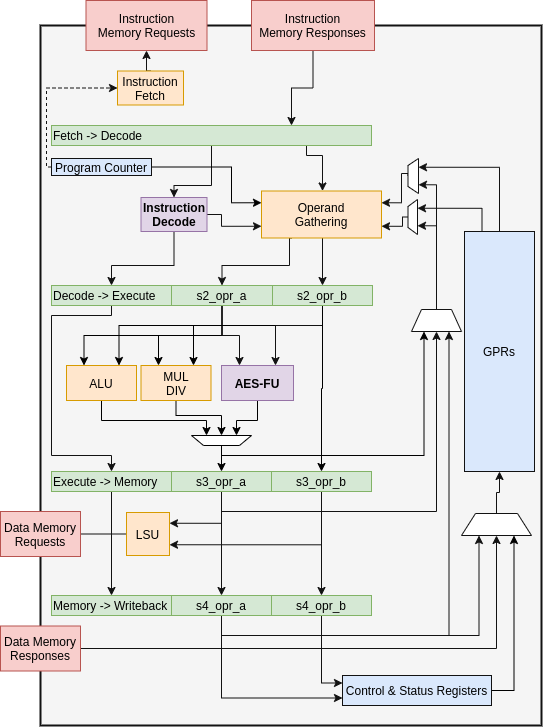
\includegraphics[scale=0.45,angle=90]{diagrams/scarv-cpu-uarch.png}
\caption{Core $2$: \CORE{2}.}
\label{fig:design:cpu_block:2}
\end{figure}

% -----------------------------------------------------------------------------

The ISE designs were evaluated using two different {\em host} cores:

\begin{itemize}
\item
    The \CORE{2} core\footnote{%
  \ifbool{anonymous}{Details of this core have been anonymised to comply with the TCHES submission guidelines.}{\url{https://github.com/scarv/scarv-cpu}}
}   is a 5-stage, in-order scalar micro-controller.
    It implements the
    {\tt rv32imc}
    instruction set: 32-bit base ISA, with the Multiply and Compressed
    ISA extensions.
    A block diagram of the core is shown in~\REFFIG{fig:design:cpu_block:2}.
    The core has separate memory interfaces for instruction and data
    accesses, with no cache hierarchy or branch prediction.
    The core implements various performance counters,
    and
    elements of the
    RISC-V Privileged Resource Architecture 
    (PRA)~\cite[Chapter 3]{RV:ISA:II:17}
    related to exception and interrupt handling.

\item
    The \CORE{1} core\cite{rocket:16} 
    is a 5-stage, in-order pipeline with a configurable cache hierarchy and
    branch predictor.
    We used both 32-bit and 64-bit variants of \CORE{1} as bases for our work.
    We configured both base designs to have a single ``big'' core, with
    no floating point support.
    ({\bf TODO:} List exactly how this configured Rocket, or just
     reproduce the chissel config code?)

\end{itemize}

Two modifications were made to the host cores to support the ISE variants:
1) The Instruction Decode module was modified to support identification and
   operand selection for the new instructions. 
2) A new ``AES'' functional unit (AES FU) was added to perform the instruction
   computations.
In the \CORE{2} core, the new block was built directly into the execution
pipeline.
For the \CORE{1}, we used the Rocket Custom Coprocessor (RoCC)
interface.
A synthesis time parameter was then added to switch between different
ISE variants for each host core.

Because all of the ISE variants read at most two,
and write one general purpose register, no new structural data-paths
were needed.
This was an important design consideration, as RISC-V tries to
aggressively follow this pattern.

% =============================================================================


% -----------------------------------------------------------------------------

\subsection{Evaluation}

\subsubsection{Hardware}
\label{sec:ise:eval:hw}
% =============================================================================

Each ISE variant was implemented and integrated into the $3$ host cores 
described in \REFSEC{sec:ise:imp}.
The variants which assume  $\RVXLEN = 32$
(\ISE{1}, \ISE{2}, \ISE{3}, and \ISE{5}) 
were evaluated wrt.
{\em both}
on the
$32$-bit \CORE{2} core
{\em  and}
$32$-bit \CORE{1} core;
the variant  which assumes $\RVXLEN = 64$
(\ISE{4})
was  evaluated wrt.
{\em only}
on the
$64$-bit \CORE{1} core.
As noted, for \ISE{1}, \ISE{2} and \ISE{5} the potential for a trade-off
between latency and area exists.  Each such case is catered for through
the consideration of two optimisation goals:
the (A)rea    goal
instantiates $1$ S-box   and has a $n$-cycle execution latency,
whereas
the (L)atency goal
instantiates $4$ S-boxes and has a $1$-cycle execution latency.

\REFTAB{tab:eval:hw} 
records
various metrics 
associated with the hardware implementations, 
arranged in two parts: 
the  left-hand part relates to each ISE in isolation,
whereas 
the right-hand part relates to each ISE integrated with a given core.
Throughout, both area (measured in NAND2 equivalent gates) and Longest 
Topological Path (LTP) are as reported by Yosys~\cite{yosys}.  We found 
that none of the ISEs affected the critical path of either the \CORE{2} 
or \CORE{1} core.
% TODO: address the issue re. Rocket area (i.e., the caches dominating)
Considering each ISE as implemented on the \CORE{1} core, we note the 
overhead wrt. area is marginal: this stems from the fact that the 
baseline area of \CORE{1} includes the data and instruction caches.

% =============================================================================


\subsubsection{Software}
\label{sec:ise:eval:sw}
% =============================================================================

To evaluate the software performance, we implemented AES 128, and
measure the static code size, instruction execution counts and cycle
counts of the Key Schedule, Encrypt and Decrypt functions.
We also separate generation of the KeySchedule for Encrypt and Decrypt.
A T-table implementation of AES (See \REFSEC{sec:bg:aes_impl_sw})
is used as a performance baseline.

\REFTAB{tab:eval:sw:size} shows the static code size for each
function.
These are measured targeting the {\tt rv32imc} base ISA for all variants,
except for V4, which targets {\tt rv64imc}.
Decryption KeySchedule entries with a $\star$ indicate that the
implementation uses the Equivalent Inverse Cipher construction
\cite[Section 5.3.5, Page 23]{FIPS:197}, meaning that the
Decrypt KeySchedule calls the Encrypt KeySchedule, then performs some
additional post processing. The code size listed is for the post processing.
The V5 Encrypt Key Schedule is split into the basic KeySchedule
operation, plus a re-arrangement of the bytes in each word to make
KeyAddition more efficient in subsequent encrypt/decrypt operations.

For the Encrypt and Decrypt functions, all versions have similar
static code size.
The 32-bit variants (V1,V2,V3,V5) all use loop-based implementations.
V1, V2, V5 implement one round per loop iteration. V3 implements two
rounds per loop iteration to avoid needless register move operations.
The 64-bit variant (V4) uses a completely un-rolled implementation.

\REFTAB{tab:eval:sw:perf:scarv}
and
\REFTAB{tab:eval:sw:perf:rocket}
give cycle and instruction counts for each
variant under the \CORE{2} and \CORE{1} cores respectively.
Each implementation uses word-aligned state, meaning the input blocks
can be loaded with $4$ load-word instructions on $32$-bit host cores,
or $2$ load-double instructions on the $64$-bit host cores.
For the Encrypt/Decrypt columns, we show instruction execution counts
and processor clock cycle measurements for a single block
encryption of AES-128.
Likewise, the KeySchedule columns are for a single AES-128 KeySchedule
operation.

% =============================================================================


\subsubsection{Discussion}
\label{sec:ise:eval:discuss}
% =============================================================================

\REFTAB{tab:eval:hw}
demonstrates that all ISE variants
imply a modest area overhead relative to their host core.
The RV32 \CORE{1} area results are not listed, as the ISE overhead compared to
the area of a synthesised Rocket Tile with caches was less than $1\%$ in all
cases.
\REFTAB{tab:eval:sw:size}
shows all ISE variants
having similarly small memory footprints in terms of both instruction code and
data.
Beyond this, and per 
\REFSEC{sec:ise:design},
the primary metric of interest is efficiency in terms of
improvement in execution latency per area:
this metric draws on data from
\REFTAB{tab:eval:hw}
plus either
\REFTAB{tab:eval:sw:perf:2}
or
\REFTAB{tab:eval:sw:perf:1}
for the \CORE{2} or \CORE{1} core respectively,
and, for each variant, is computed by dividing the improvement in execution 
latency (relative to the T-table baseline) by the normalised area (i.e., the 
ISE area column of \REFTAB{tab:eval:hw}). We deliberately omit the area of
the host core from this calculation, as this fixed overhead dominates the
final value and detracts from the comparison between ISEs themselves.

\REFTAB{tab:eval:results} 
captures the results for the \CORE{1} core, although the same conclusion can 
be drawn for the \CORE{2} core.  Qualitatively, we place more of a weight on 
\ALG{Enc} 
and 
\ALG{Dec} 
vs.
\ALG{Enc-KeyExp} 
and 
\ALG{Dec-KeyExp},
because
typically many \ALG{Enc} or \ALG{Dec} operations are performed per
\ALG{KeyExp}.
For a $32$-bit core, our conclusion is that
\ISE{3} 
is the best option.
Despite not being the fastest (by a small margin), it is the most efficient,
and simplest to implement.
The area optimised \ISE{2} implementation sometimes comes close in
efficiency, but requires a more complex multi-cycle implementation
in this case.
For a $64$-bit core,
\ISE{4} 
is the best option, which is somewhat obvious because it specifically makes
use of the wider data-path.
With reference to
\REFTAB{tab:eval:sw:perf:1}, 
note that the number of cycles per instruction executed is relatively low.
This fact stems from use of the ROCC interface, in that forwarding of the 
result from an ISE instruction (that uses the ROCC) incurs an overhead vs. 
an ISE instruction; fine-grained integration of the AES-FU could therefore
incrementally improve the results.

We believe it is sensible to standardise different ISEs for the
RV32 and RV64 base ISAs.
This allows each ISE design to better suit the constraints of each
base ISA.
In the RV32 case, this acknowledges that such cores will most often
appear in resource-constrained, embedded or IoT class devices.
Hence, the most efficient ISE design is appropriate.
For necessarily larger RV64-based designs, it makes sense to take advantage
of the wider data-path, and acknowledge that these are more likely to
be application class cores. Hence, they will place a higher value
on performance than area-efficiency.

% -----------------------------------------------------------------------------

\begin{adjustbox}{center,caption={Hardware implementation metrics 
                                  (e.g., area and Circuit Depth)
                                  for each ISE variant.
                                 },label={tab:eval:hw},float={table}[!p]}
\centering
\begin{tabular}{|c|c@{\;}c|rr|rr|}
\hline
  \multicolumn{1}{|c|}{ISA}
& \multicolumn{1}{ c }{Variant}
& \multicolumn{1}{ c|}{(Goal)}
& \multicolumn{1}{ c|}{             ISE area}
& \multicolumn{1}{ c|}{             ISE Circuit Depth}
& \multicolumn{2}{ c|}{\CORE{2} $+$ ISE area}
\\
\hline
\hline
 RV32IMC &          &     &              &            &       37375 &       (1.00$\times$) \\
 RV32IMC & \ISE{1}  & (L) &        3472  & \bftab 19  &       41723 &       (1.12$\times$) \\
 RV32IMC & \ISE{1}  & (A) &        2174  &        22  &       40161 &       (1.07$\times$) \\
 RV32IMC & \ISE{2}  & (L) &        3547  & \bftab 19  &       41199 &       (1.10$\times$) \\
 RV32IMC & \ISE{2}  & (A) &        1381  &        21  &       38885 &       (1.04$\times$) \\
 RV32IMC & \ISE{3}  &     & \bftab 1157  &        30  &\bftab 38610 &\bftab (1.03$\times$) \\
 RV32IMC & \ISE{5}  & (L) &        4121  &        22  &       42070 &       (1.13$\times$) \\
 RV32IMC & \ISE{5}  & (A) &        1927  &        23  &       39251 &       (1.05$\times$) \\
\hline
\hline
  \multicolumn{1}{|c|}{ISA}
& \multicolumn{1}{ c }{Variant}
& \multicolumn{1}{ c|}{(Goal)}
& \multicolumn{1}{ c|}{             ISE area}
& \multicolumn{1}{ c|}{             ISE Circuit Depth}
& \multicolumn{2}{ c|}{\CORE{1} $+$ ISE area}
\\
\hline
 RV64IMC &          &     &$          $&$          $&$   3717607 $&$     (1.000\times)$ \\
 RV64IMC & \ISE{4}  &     &$     8312 $&$       27 $&$   3733786 $&$     (1.004\times)$ \\
\hline
\end{tabular}
\end{adjustbox}

\begin{adjustbox}{center,caption={Software implementation metrics 
                                  (i.e., memory footprint measured in bytes)
                                  for each ISE variant.
                                 },label={tab:eval:sw:size},float={table}[!p]}
\centering
\begin{tabular}{|c|c|r|r|r|r|r|}
\hline
  \multicolumn{1}{|c|}{ISA}
& \multicolumn{1}{ c|}{Variant}
& \multicolumn{1}{ c|}{$\ALG{Enc}$}
& \multicolumn{1}{ c|}{$\ALG{Dec}$}
& \multicolumn{1}{ c|}{$\ALG{Enc-KeyExp}$}
& \multicolumn{1}{ c|}{$\ALG{Dec-KeyExp}$}
& \multicolumn{1}{ c|}{.data} 
\\
\hline
\hline
%RV32IMC & Byte    &            &           &      312 &        0 &  522 \\
 RV32IMC & T-table &       804  &       804 &      154 &      174 & 5120 \\
 RV32IMC & \ISE{1} &       424  &       424 &\bftab 68 &        0 &   10 \\
 RV32IMC & \ISE{2} &\bftab 234  &\bftab 238 &\bftab 68 &       62 &   10 \\
 RV32IMC & \ISE{3} &       290  &       290 &       86 &       64 &   10 \\
 RV32IMC & \ISE{5} &       266  &       278 &      290 &        0 &   10 \\
\hline
 RV64IMC & \ISE{4} &       268  &       268 &      168 &      100 &    0 \\
\hline
\end{tabular}
\end{adjustbox}

\begin{adjustbox}{center,caption={Execution metrics
                                  for each ISE variant on the \CORE{2} core.
                                  Note that the $64$-bit \ISE{4} is absent, since there is no $64$-bit \CORE{2} core.
                                 },label={tab:eval:sw:perf:2},float={table}[!p]}
\centering
\begin{tabular}{|c|c@{\;}c|rr|rr|rr|rr|}
\hline
  \multicolumn{1}{|c|}{ISA}
& \multicolumn{1}{ c }{Variant}
& \multicolumn{1}{ c|}{(Goal)}
& \multicolumn{2}{ c|}{$\ALG{Enc}$}
& \multicolumn{2}{ c|}{$\ALG{Dec}$}
& \multicolumn{2}{ c|}{$\ALG{Enc-KeyExp}$}
& \multicolumn{2}{ c|}{$\ALG{Dec-KeyExp}$}
\\
\cline{4-11}
&
&
& \multicolumn{1}{ c|}{iret}
& \multicolumn{1}{ c|}{cycles}
& \multicolumn{1}{ c|}{iret}
& \multicolumn{1}{ c|}{cycles}
& \multicolumn{1}{ c|}{iret}
& \multicolumn{1}{ c|}{cycles}
& \multicolumn{1}{ c|}{iret}
& \multicolumn{1}{ c|}{cycles}
\\
\hline
\hline
%RV32IMC & Byte    &     &            &            &            &            &            &            &            &            \\
 RV32IMC & T-table &     &       998  &      1076  &       998  &      1103  &       466  &       554  &      1747  &      2346  \\ 
 RV32IMC & \ISE{1} & (L) &       518  &       593  &       518  &       607  &\bftab 198  &\bftab 291  &\bftab 204  &\bftab 310  \\
 RV32IMC & \ISE{1} & (A) &       518  &       753  &       518  &       775  &\bftab 198  &       331  &\bftab 204  &       350  \\
 RV32IMC & \ISE{2} & (L) &\bftab 221  &       301  &\bftab 222  &       303  &\bftab 198  &       302  &       335  &       616  \\
 RV32IMC & \ISE{2} & (A) &\bftab 221  &       538  &\bftab 222  &       540  &\bftab 198  &       332  &       335  &       754  \\
 RV32IMC & \ISE{3} &     &       238  &\bftab 291  &       238  &\bftab 286  &       219  &       312  &       659  &      1118  \\
 RV32IMC & \ISE{5} & (L) &       233  &       304  &       233  &       309  &       332  &       447  &       338  &       466  \\
 RV32IMC & \ISE{5} & (A) &       233  &       556  &       233  &       550  &       332  &       477  &       338  &       496  \\
\hline
\end{tabular}                
\end{adjustbox}

\begin{adjustbox}{center,caption={Execution metrics
                                  for each ISE variant on the \CORE{1} core.
                                  Note that the $64$-bit \ISE{4} uses the $64$-bit \CORE{1} core; all others use the $32$-bit \CORE{1} core.
                                 },label={tab:eval:sw:perf:1},float={table}[!p]}
\centering
\begin{tabular}{|c|c@{\;}c|rr|rr|rr|rr|}
\hline
  \multicolumn{1}{|c|}{ISA}
& \multicolumn{1}{ c }{Variant}
& \multicolumn{1}{ c|}{(Goal)}
& \multicolumn{2}{ c|}{$\ALG{Enc}$}
& \multicolumn{2}{ c|}{$\ALG{Dec}$}
& \multicolumn{2}{ c|}{$\ALG{Enc-KeyExp}$}
& \multicolumn{2}{ c|}{$\ALG{Dec-KeyExp}$}
\\
\cline{4-11}
&
&
& \multicolumn{1}{ c|}{iret}
& \multicolumn{1}{ c|}{cycles}
& \multicolumn{1}{ c|}{iret}
& \multicolumn{1}{ c|}{cycles}
& \multicolumn{1}{ c|}{iret}
& \multicolumn{1}{ c|}{cycles}
& \multicolumn{1}{ c|}{iret}
& \multicolumn{1}{ c|}{cycles}
\\
\hline
\hline
%RV32IMC & Byte    &     &            &            &            &            &            &            &            &            \\
 RV32IMC & T-table &     &       948  &      1143  &       949  &      1025  &       444  &       478  &      1726  &      1977  \\
 RV32IMC & \ISE{1} & (L) &       528  &       685  &       529  &       680  &\bftab 212  &       341  &\bftab 214  &\bftab 290  \\
 RV32IMC & \ISE{1} & (A) &       528  &       804  &       529  &       744  &\bftab 212  &       357  &\bftab 214  &       335  \\
 RV32IMC & \ISE{2} & (L) &\bftab 231  &\bftab 359  &\bftab 233  &       368  &\bftab 212  &\bftab 315  &       350  &       508  \\
 RV32IMC & \ISE{2} & (A) &\bftab 231  &       511  &\bftab 233  &       520  &       212  &       345  &       350  &       646  \\
 RV32IMC & \ISE{3} &     &       253  &       445  &       254  &       445  &       233  &       470  &       674  &      2425  \\
 RV32IMC & \ISE{5} & (L) &       243  &       414  &       244  &\bftab 319  &       346  &       427  &       348  &       424  \\
 RV32IMC & \ISE{5} & (A) &       243  &       585  &       244  &       543  &       346  &       504  &       348  &       454  \\
\hline
 RV64IMC & \ISE{4} &     &        81  &       119  &        82  &       125  &        66  &       204  &       136  &       306  \\
\hline
\end{tabular}
\end{adjustbox}

% -----------------------------------------------------------------------------

\begin{adjustbox}{center,caption={Comparison of improvement per unit-area 
                                  for each ISE variant. 
                                 },label={tab:eval:results},float={table}[!t]}
\centering
\begin{tabular}{|c|c@{\;}c|rr|rr|rr|rr|}
\hline
  \multicolumn{1}{|c|}{ISA}
& \multicolumn{1}{ c }{Variant}
& \multicolumn{1}{ c|}{(Goal)}
& \multicolumn{2}{ c|}{$\ALG{Enc}$}
& \multicolumn{2}{ c|}{$\ALG{Dec}$}
& \multicolumn{2}{ c|}{$\ALG{Enc-KeyExp}$}
& \multicolumn{2}{ c|}{$\ALG{Dec-KeyExp}$}
\\
\cline{4-11}
&
&
& \multicolumn{1}{ c|}{iret}
& \multicolumn{1}{ c|}{cycles}
& \multicolumn{1}{ c|}{iret}
& \multicolumn{1}{ c|}{cycles}
& \multicolumn{1}{ c|}{iret}
& \multicolumn{1}{ c|}{cycles}
& \multicolumn{1}{ c|}{iret}
& \multicolumn{1}{ c|}{cycles}
\\
\hline
\hline
RV32IMC & \ISE{1} & (L) &       4.61  &       4.34  &       4.61  &       4.35  &       5.39  &       6.06  &      20.50  &      18.12   \\
RV32IMC & \ISE{1} & (A) &       7.37  &       5.46  &       7.37  &       5.44  &       8.61  &       6.40  &\bftab32.74  &\bftab25.63   \\
RV32IMC & \ISE{2} & (L) &      10.58  &       8.38  &      10.53  &       8.53  &       5.28  &       4.30  &      12.22  &       8.92   \\
RV32IMC & \ISE{2} & (A) &      27.18  &      12.04  &      27.06  &      12.29  &      13.56  &      10.04  &      31.39  &      18.73   \\
RV32IMC & \ISE{3} &     &\bftab30.12  &\bftab26.56  &\bftab30.12  &\bftab27.71  &\bftab14.63  &\bftab12.76  &      19.04  &      15.08   \\
RV32IMC & \ISE{5} & (L) &       8.64  &       7.14  &       8.64  &       7.20  &       2.71  &       2.50  &      10.43  &      10.15   \\
RV32IMC & \ISE{5} & (A) &      18.48  &       8.35  &      17.64  &       8.30  &       5.79  &       5.01  &      22.29  &      20.40   \\
\hline
RV64IMC & \ISE{4} &     &      12.32  &       9.04  &      12.17  &       8.82  &       6.76  &       2.72  &      12.85  &       7.67   \\
\hline
\end{tabular}
\end{adjustbox}

% =============================================================================


% =============================================================================

\section{Using ISEs to implement AES-GCM}
\label{sec:gcm}
% =============================================================================

\begin{adjustbox}{center,caption={Instruction    counts for multiplication in $\F_{2^{128}}$ as used by \ALG{GHASH}.
                                 },label={tab:gcm:instrs},float={table}[!t]}
\centering
\begin{tabular}{|c|c|c|rrrrrr|}
\hline
ISA    & Karatsuba & Reduce & \VERB{grev}
                            & \VERB{xor}
                            & \VERB{s[lr]li}
                            & \VERB{clmul} 
                            & \VERB{clmulh}
                            & Total \\
\hline
\hline
RV32IB &        no &    mul &$  4$&$ 36$&$  0$&$ 20$&$ 20$&$ 80$ \\
RV32IB &        no &  shift &$  4$&$ 56$&$ 24$&$ 16$&$ 16$&$116$ \\
RV32IB &       yes &    mul &$  4$&$ 52$&$  0$&$ 13$&$ 13$&$ 82$ \\
RV32IB &       yes &  shift &$  4$&$ 72$&$ 24$&$  9$&$  9$&$118$ \\
\hline
RV64IB &        no &    mul &$  2$&$ 10$&$  0$&$  6$&$  6$&$ 24$ \\
RV64IB &        no &  shift &$  2$&$ 20$&$ 12$&$  4$&$  4$&$ 42$ \\
RV64IB &       yes &    mul &$  2$&$ 14$&$  0$&$  5$&$  5$&$ 26$ \\
RV64IB &       yes &  shift &$  2$&$ 24$&$ 12$&$  3$&$  3$&$ 44$ \\
\hline
\end{tabular}
\end{adjustbox}

\begin{adjustbox}{center,caption={Modelled cycle counts for multiplication in $\F_{2^{128}}$ as used by \ALG{GHASH}.
                                 },label={tab:gcm:cycles},float={table}[!t]}
\centering
\begin{tabular}{|c|c|c|rrrr|}
\hline
ISA    & Karatsuba & Reduce & $1$-cycle       & $2$-cycle       & $3$-cycle       & $6$-cycle       \\
       &           &        & \VERB{clmul[h]} & \VERB{clmul[h]} & \VERB{clmul[h]} & \VERB{clmul[h]} \\
\hline
\hline
RV32IB &        no &    mul &$      {\bf  80}$&$           120 $&$           160 $&$           280 $\\
RV32IB &        no &  shift &$           116 $&$           148 $&$           180 $&$           276 $\\
RV32IB &       yes &    mul &$            82 $&$      {\bf 108}$&$      {\bf 134}$&$           212 $\\
RV32IB &       yes &  shift &$           118 $&$           136 $&$           154 $&$      {\bf 208}$\\
\hline
RV64IB &        no &    mul &$      {\bf  24}$&$      {\bf  36}$&$            48 $&$            84 $\\
RV64IB &        no &  shift &$            42 $&$            50 $&$            58 $&$            82 $\\
RV64IB &       yes &    mul &$            26 $&$      {\bf  36}$&$      {\bf  46}$&$            76 $\\
RV64IB &       yes &  shift &$            44 $&$            50 $&$            56 $&$      {\bf  74}$\\
\hline
\end{tabular}
\end{adjustbox}

% -----------------------------------------------------------------------------

Per
\REFSEC{sec:bg:aes_usage},
The Galois/Counter Mode (GCM)
~\cite{NIST:sp.800.38d}
is a block cipher mode of operation which 
supports authenticated encryption.
AES-GCM refers to an instantiation using AES as the underlying block cipher, 
which is the only case mandated by TLS 1.3~\cite[Section 9.1]{rfc:8446}; the
importance of this construction means GCM and AES are frequently considered 
together from an implementation and evaluation perspective.
Again 
per
\REFSEC{sec:bg:aes_usage},
the computational core of AES-GCM is formed from 
1) \ALG{GCTR}, i.e., AES encryption,
   and
2) \ALG{GHASH}.
Since we dealt with efficient implementation of AES and hence \ALG{GCTR} in
\REFSEC{sec:ise}, we turn our attention to \ALG{GHASH}.  
Rather than further 
embellish the ISE for AES, we instead focus on use of the existing
standard 
B~\cite[Section 17]{RV:ISA:I:19}
extension.

% -----------------------------------------------------------------------------

\paragraph{Implementation.}

\ALG{GHASH}~\cite[Section 6.4]{NIST:sp.800.38d} is a universal hash defined 
over $\F_{2^{128}}$.
Conversion of the input into the correct endian'ness can be realised using
the 
\VERB{grev} (or generalised reverse)
instruction,
which reverses the bits in each byte of an input word:
$4$ (resp. $2$) 
\VERB{grev} 
instructions are therefore required on RV32IB (resp. RV64IB).
Beyond this, operations in $\F_{2^{128}}$ dominate.
Addition       in $\F_{2^{128}}$ 
is trivial, since addition modulo $2$ is equivalent to XOR: this
$4$ (resp. $2$) 
\VERB{xor} 
instructions are therefore required on RV32IB (resp. RV64IB).
Multiplication in $\F_{2^{128}}$ 
can be decomposed into two steps:
1) a $( 128 \time 128 )$-bit polynomial multiplication, 
   followed by 
2) a reduction of the $256$-bit result modulo
   $
   \IND{x}^{128} + \IND{x}^{7} + \IND{x}^{2} + \IND{x} + 1 .
   $
The first  step 
can be realised using pairs of ``carry-less'' multiplication instructions
\VERB{clmul} and \VERB{clmulh}.
These instructions compute the least-significant (resp. most-significant) 
half of a carry-less product (i.e., product over $\F_2$); pairs of 
\VERB{clmul} and \VERB{clmulh}
should be scheduled adjacently, st. capable micro-architectures are able 
to fuse them.
Use of a school-book approach 
requires
$16$ (resp. $4$) such pairs 
on RV32IB (resp. RV64IB);
optimisation using the Karatsuba-Ofman method
requires
$ 9$ (resp. $3$) such pairs 
on RV32IB (resp. RV64IB) 
plus some additional \VERB{xor} instructions.
The second step
can be realised using two approaches:
1) a          shift-based reduction, made possible by the low Hamming weight of the primitive polynomial,
   or
2) a multiplication-based reduction, analogous to the Montgomery or Barret methods.
Overall, the most efficient approach on the relative execution latencies of
\VERB{clmul} and \VERB{clmulh}
vs.
\VERB{xor} and \VERB{s[lr]li};
We note that 
\VERB{clmul} and \VERB{clmulh}
{\em must} exhibit data-oblivious execution latency 
(e.g., avoid data-dependent optimisations such as early-termination)
to avoid associated side-channel attack (cf.~\cite{GOPT:09}).

% -----------------------------------------------------------------------------

\paragraph{Discussion.}

\REFTAB{tab:gcm:instrs} 
lists instruction counts for 
multiplication in $\F_{2^{128}}$,
as implemented using different combinations of the base ISA, and approaches
for the polynomial multiplication and reduction steps.
\REFTAB{tab:gcm:cycles} 
then model the execution latency 
(measured in cycles)
assuming that \VERB{grev}, \VERB{xor}, and \VERB{s[lr]li} take $1$ cycle.
Although the model only considers an in-order core in line with those used
in \REFSEC{sec:ise} and is focused on execution latency
(vs. other pertinent metrics, such as code footprint),
there are two obvious conclusions:
1) iff.
   \VERB{clmul} and \VERB{clmulh}
   have $2$ (or more) times the latency of
   \VERB{xor} and \VERB{s[lr]li},
   a 
   Karatsuba-Ofman 
   polynomial multiplication
   is preferable,
   and
2) if
   \VERB{clmul} and \VERB{clmulh}
   have $6$ (or more) times the latency of
   \VERB{xor} and \VERB{s[lr]li},
   a shift-based 
   reduction 
   is preferable.

% =============================================================================


% =============================================================================

\section{Hardening an ISE for AES against DPA attack}
\label{sec:sca}

In embedded, IoT class devices to which an attacker may have
physical access,
Differential Power Analysis (DPA) attacks on cryptographic implementations
\cite{KJJ:99} can be devastating.
While ISEs give a notable increase in efficiency, they can also create
attractive targets for DPA attacks.
This stems from there being only one way to sensibly implement
AES using the ISE and the ISE having very well defined behaviour.
This reduces the number of target variables or
implementation choices an attacker needs to consider.
It is then important to consider how an implementer might
further extend a cryptographic ISE to secure it against DPA attacks.
While our focus here is on DPA attacks, we note that Differential
Electro-Magnetic Analysis attacks are exploited and countered using
similar techniques to DPA.

Having identified ISE \ISE{3} as a strong standardisation candidate
for embedded $32$-bit RISC-V cores, we take a hardware/software co-design
approach to extending the ISE, adding $1$st order DPA side-channel
resistance.

\subsection{Design}

We base our design on boolean masking, and represent the secret
key as two Boolean masked shares.

An implementation of the AES block encrypt/decrypt function 
using \ISE{3} requires eight $\GPR$s:
four for the current round state and
four to load the next round key
and
then accumulate the next round state.
See \REFFIG{fig:v3:round} for an AES round function implementation
using \ISE{3}.
Storing shares of each secret variable
in the General Purpose Register (GPR) file is un-reasonable,
requiring drastic modifications to the instruction definitions and
register file to read four registers (two sources, of two shares each) and
write two registers.
This would break the RISC-V $2$-read-$1$-write principle.
Storing corresponding shares in the GPRs is also a security
risk, as they may be accidentally combined due to
careless instruction use, or implicit register accesses by the
CPU micro-architecture.

Instead, we define a new, $8$-element ``Mask Register File'' (MRF).
Each mask register $M_i$ is $w=32$-bits wide, and stores the mask for
one of the GPRs.
We use a fixed mapping between GPRs and mask registers;
not all GPRs have a corresponding mask register.
We use the mapping $\{a0..a3,t0..t4\} \Rightarrow \{m0..m7\}$.

Share $0$ of each secret value is loaded into the GPRs using the
standard RISC-V Load Word ({\tt lw}) instruction.
We define a new Load Mask instruction {\tt lm rd, offset(rs1)} which
loads {\em the mask for GPR {\tt rd}}
(i.e. Share $1$)
from memory into the corresponding MRF entry.
A corresponding Store Mask instruction {\tt sm rs2, offset(rs1)} writes
the mask corresponding to GPR {\tt rs2} to memory.
The {\tt sm} instruction is only used for context switches, and
destructively reads the MRF register value to prevent it being
leaked to other applications running on the same core.\footnote{
    In this case, destructive could mean set to zero (which could
    leak the hamming weight of the mask) or randomising its value.}
We require the secret values be stored in shared form in memory
(rather than splitting them into shares upon being loaded)
to extend the SCA protection boundary outside the CPU.
Otherwise, the hamming weight of unmasked secret values would be
leaked by memory-hierarchy registers outside the CPU.
Executing an {\tt lm} instruction such that {\tt rd} does not map to
a mask register raises an illegal opcode exception.
Likewise for {\tt sm} and {\tt rs2}.

When an ISE instruction is executed and its $\GPR$ source
registers map to an MRF register, both the $\GPR$s and MRF are
read simultaneously and fed to the AES functional unit.
If any $\GPR$ source does not map to an MRF register, we assume that
operand is unmasked and represent the other share as $0$.

Within the AES-FU the instruction result is computed entirely in a
masked representation.
The result shares are then re-masked before being written back to the
$\GPR$s and MRF.
This is necessary, because \ISE{3} instructions are designed
such that {\tt rs1=rd} for all use cases.
Without re-masking, overwriting a source with the result could cause 
$1$'st order hamming-distance leakage.

If the destination $\GPR$ has a corresponding
mask register, share $0$ is stored in the $\GPR$s and share $1$ in the MRF.
If the destination $\GPR$ does not map to a mask register, the result is
written to the GPR unmasked.
This means that in the final encrypt/decrypt round, we can optionally obtain
the unmasked results without having to store the shares to memory,
load them back and unmask them.

\subsection{Implementation}

We used the \CORE{2} core as the basis for our side-channel secure
implementation of \ISE{3}.
\REFFIG{fig:core:2:secure} shows a block diagram of the modifications
made to the core, and which data-paths carry masked data.
To avoid accidental unmasking of the two shares,
Share $1$ is stored in {\em bit-reversed} form in the MRF and pipeline
registers.
This means that any accidental multiplexing between pipeline operand
registers causes toggles between non-corresponding bits of each share.
Share $1$ is only un-reversed immediately prior to entering the
AES functional unit, and is re-reversed before exiting it.
Bit-reversal has zero logic gate cost and some minor routing complexity.

While the architectural state stores a $2$-share representation
of the secret material, we use a $3$-share implementation of the
AES S-box.
This was driven by experiments showing 
leakage from a $2$-share design in our FPGA platform.
The additional share is generated by a simple $32$-bit LFSR and added
dynamically by the hardware, and is never visible to the programmer.
This is suitable for a proof of concept (evident in the experimental
results) but would need to be used in conjunction with a true random
number source (e.g., a set of ring-oscillators) in a deployed system.
Only the S-box is implemented using $3$-shares.
Subsequent \AESFUNC{MixColumns} logic is only implemented using $2$ shares.

\subsection{Evaluation}

The modified \CORE{2} core was implemented on a
Sasebo GIII \cite{HKSS:12}
side-channel analysis platform, containing two Xilinx FPGAs:
a Kintex-7 
(model {\tt xc7k160tfbg676})
target
and
a supporting Spartan-6
(model {\tt xc6slx45}).
Only the Kintex-7 was used.
The design was synthesised using Xilinx Vivado 2019.2 with
default synthesis and implementation strategies.
The Kintex-7 FPGA uses a 200MHz differential external clock source, which is
transformed into a 50MHz internal clock used by the entire design.

Trace capture uses a standard pipeline of components:
a MiniCircuits BLK+89 D/C blocker,
an Agilent 8447D amplifier (with a $\SI{100}{\kilo\hertz}$ to $\SI{1.3}{\giga\hertz}$ range, and $\SI{25}{\decibel}$ gain),
and
a  PicoScope 5000 series oscilloscope using a
250 MHz sample rate, with a 12-bit resolution.

We performed a generic randomised plaintext
Test Vector Leakage Assessment (TVLA) \cite{TVLA:13}
flow to evaluate the effectiveness of the side-channel hardened implementation,
using the AES-128 block encrypt function as the target operation.
The unprotected and protected implementation results are shown in
\REFFIG{fig:sca:unprotected} and
\REFFIG{fig:sca:protected} respectively.
The protected implementation is effective at removing $1$st
order side-channel leakage up to $100$K traces.
The peaks at the beginning and end of \REFFIG{fig:sca:protected}
are caused by the unmasked block input and output data being loaded/stored.

\REFTAB{tab:sca:sw-hw} shows the hardware and software overheads.
The ISE Size/LTP rows are inclusive of the S-box Size/LTP rows.
Likewise, the CPU Size rows are inclusive of the ISE Size rows.
The static code size and instruction count overheads are
$\approx 20\%$: considerably less than a non-ISE-based software masking
approach.
The hardware overheads are dominated by the increased size of the
S-box (owing to the 3-share design), and the MRF.
Although the overhead to the dedicated
ISE logic is $~4x$, this drops to $~1.2x$ when the entire
CPU sub-system is considered.
Measured against an entire SoC, the overheads are modest.

\begin{table}[]
\centering
\begin{tabular}{|l|r|r|r|}
\hline
Metric  & Unprotected & Protected  & Overhead \\
\hline
\hline
Static Code Size (Bytes)        & 290         & 358    & $1.23\times$   \\
Instructions Executed           & 238         & 287    & $1.21\times$   \\
CPU Clock Cycles                & 291         & 331    & $1.14\times$   \\
\hline
S-box Size (NAND2 Equivalent)   & 554         & 3245   & $5.86\times$   \\
S-box circuit depth             & 19          & 22     & $1.16\times$   \\
ISE Size (NAND2 Equivalent)     & 1157        & 4616   & $3.99\times$   \\
ISE circuit depth               & 30          & 37     & $1.23\times$   \\
CPU Size (NAND2 Equivalent)     & 38610       & 45141  & $1.16\times$   \\
CPU Size  LUTs                  & 4017        & 4956   & $1.23\times$   \\
CPU Size  FFs                   & 2078        & 2420   & $1.16\times$   \\
FPGA Timing Slack @50MHz        & 8.12ns      & 7.05ns & $0.87\times$   \\
\hline
\end{tabular}
\caption{
Software and hardware overheads for the protected ISE implementation
of AES-128 block encryption.
The ``ISE Size'' row does not include the cost of the mask register file
for the protected implementation;
this is included in the CPU size measurements, since the exact method
of mask delivery and storage is an implementation option.
}
\label{tab:sca:sw-hw}
\end{table}

\begin{figure}
\centering
\begin{subfigure}[t]{0.95\textwidth}
\centering
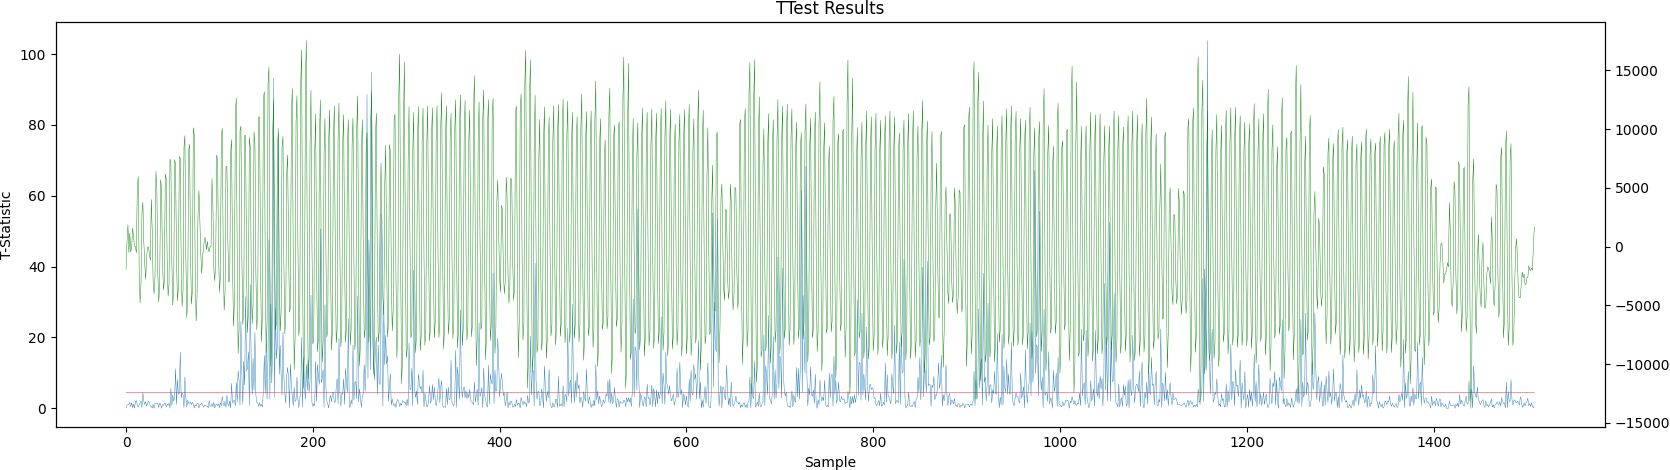
\includegraphics[width=\textwidth]{graphs/aes-vanilla-enc-default-ttest.png}
\caption{
    Un-protected implementation TVLA results after $10$K traces.
}
\label{fig:sca:unprotected}
\end{subfigure}
\begin{subfigure}[t]{0.95\textwidth}
\centering
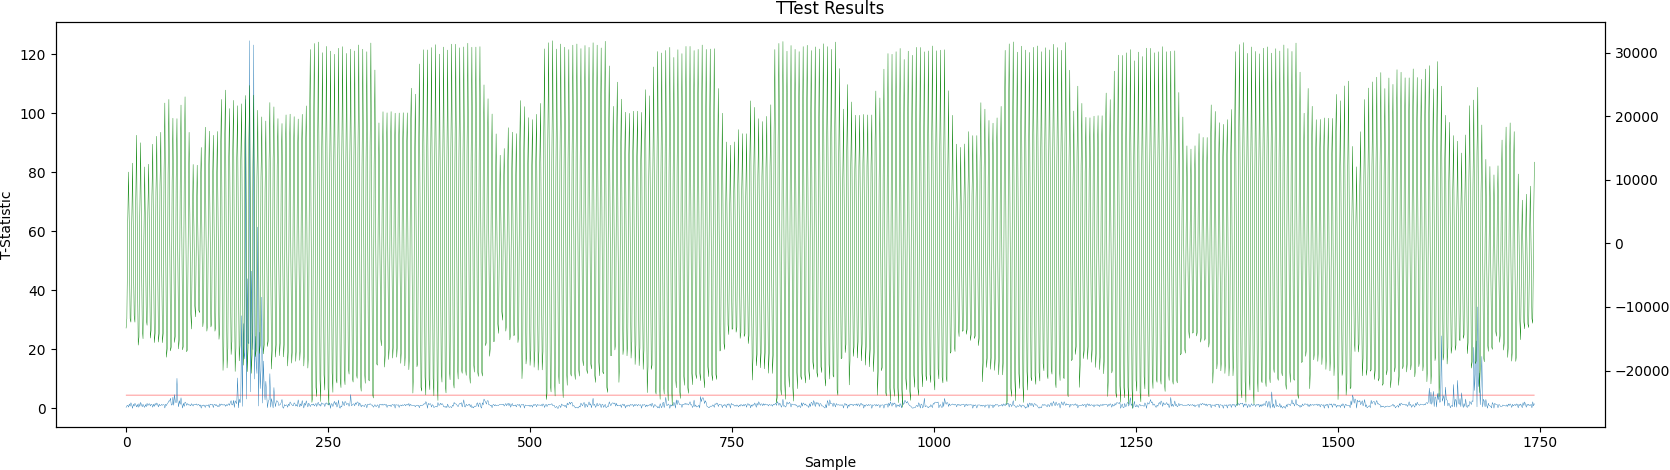
\includegraphics[width=\textwidth]{graphs/aes-secure-enc-default-ttest.png}
\caption{
    Side-channel protected implementation TVLA results after $100$K traces.
}
\label{fig:sca:protected}
\end{subfigure}
\caption{
TVLA results for the baseline and protected implementations.
The blue trace is the absolute result of the TVLA evaluation, the green
trace is the average power consumption for each TVLA trace set.
}
\end{figure}


% =============================================================================

\section{Conclusion}
\label{sec:outro}
% =============================================================================

{\bf TODO:}

% =============================================================================


% ============================================================================

\ifbool{anonymous}{}{%
\section*{Acknowledgements}

We would like to thank the anonymous reviewers for their helpful and 
constructive comments.
This work has been supported in part by EPSRC via grant EP/R012288/1, 
under the RISE (\url{http://www.ukrise.org}) programme.
}%

% =============================================================================

\bibliographystyle{alpha}
\bibliography{paper}

% =============================================================================

\appendix

\clearpage
\section{\ISE{1}:       additional technical detail}
\label{sec:pseudo:v1}
% =============================================================================

\begin{figure}[!h]
\begin{lstlisting}[language=pseudo,style=block]
saes.v1.encs rd, rs1 : v1.SubBytes(rd, rs1, fwd=1)
saes.v1.decs rd, rs1 : v1.SubBytes(rd, rs1, fwd=0)
saes.v1.encm rd, rs1 : v1.MixColumn(rd, rs1, fwd=1)
saes.v1.decm rd, rs1 : v1.MixColumn(rd, rs1, fwd=0)
\end{lstlisting}
\caption{
  Instruction mnemonics, and their mapping onto pseudo-code functions, for \ISE{1}.
}
\label{fig:v1:mnemonics}
\end{figure}

\begin{figure}[!h]
\begin{lstlisting}[language=pseudo,style=block]
v1.SubByte(rd, rs1, fwd):
    rd.8[i] = AESSBox[rs1.8[i]] if fwd else AESInbSBox[rs1.8[i]] for i=0..3

v1.MixColumn(rd, rs1, fwd)
    for i=0..3:
        tmp.32  = ROTL32(rs1.32, 8*i)
        rd.8[i] = AESMixColumn(tmp.32) if fwd else AESInvMixColumn(tmp.32)
\end{lstlisting}
\caption{
  Instruction pseudo-code functions for \ISE{1}.
}
\label{fig:v1:pseudo}
\end{figure}

\begin{figure}[!h]
\begin{lstlisting}[language=pseudo,style=block]
lw           a0,  0(a4)       // Load Round Key
lw           a1,  4(a4)
lw           a2,  8(a4)
lw           a3, 12(a4)
xor          t0, t0, a0       // Add Round Key
xor          t1, t1, a1
xor          t2, t2, a2
xor          t3, t3, a3
saes.v1.encs a0, t0           // SubBytes
saes.v1.encs a1, t1
saes.v1.encs a2, t2
saes.v1.encs a3, t3
// Shift rows omitted - 31 Base ISE shift / or instructions.
saes.v1.encm t0, t0           // MixColumns
saes.v1.encm t1, t1
saes.v1.encm t2, t2
saes.v1.encm t3, t3
\end{lstlisting}
\caption{
  An AES encryption round implemented using \ISE{1}.
}
\label{fig:v1:round}
\end{figure}

\newpage

\begin{figure}[!h]
\centering
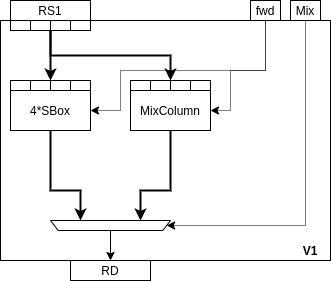
\includegraphics[width={0.5\textwidth}]{diagrams/ise-datapath-v1.png}
\caption{
  A diagramatic description of the functional unit required to support \ISE{1}.
}
\label{fig:v1:fu}
\end{figure}

% =============================================================================

\clearpage
\section{\ISE{2}:       additional technical detail}
\label{sec:pseudo:v2}
% =============================================================================

\begin{figure}[!h]
\begin{lstlisting}[language=pseudo,style=block]
saes.v2.encs rd, rs1, rs2 : v2.SubBytes(rd, rs1, rs2, fwd=1)
saes.v2.decs rd, rs1, rs2 : v2.SubBytes(rd, rs1, rs2, fwd=0)
saes.v2.encm rd, rs1, rs2 : v2.MixColumns(rd, rs1, rs2, fwd=1)
saes.v2.decm rd, rs1, rs2 : v2.MixColumns(rd, rs1, rs2, fwd=0)
\end{lstlisting}
\caption{
  Instruction mnemonics, and their mapping onto pseudo-code functions, for \ISE{2}.
}
\label{fig:v2:mnemonics}
\end{figure}

\begin{figure}[!h]
\begin{lstlisting}[language=pseudo,style=block]
v2.SubBytes(rd, rs1, rs2, fwd):
  t1.32  = {rs1.8[0], rs2.8[1], rs1.8[2], rs2.8[3]}
  rd.8[i]= AESSBox[t1.8[i]] if fwd else AESInvSBox[t1.8[i]] for i=0..3

v2.MixColumns(rd, rs1, rs2, fwd):
  t1.32  = {rs1.8[0], rs1.8[1], rs2.8[2], rs2.8[3]}
  for i=0..3:
      tmp.32 = ROTL32(rs1.32, 8*i)
      rd.8[i]= AESMixColumn(tmp.32) if fwd else AESInvMixColumn(tmp.32)
\end{lstlisting}
\caption{
  Instruction pseudo-code functions for \ISE{2}.
}
\label{fig:v2:pseudo}
\end{figure}

\begin{figure}[!h]
\begin{lstlisting}[language=pseudo,style=block]
lw              a0,  0(a4)     // Load Round Key
lw              a1,  4(a4)
lw              a2,  8(a4)
lw              a3, 12(a4)
xor             t0, t0, a0     // Add Round Key
xor             t1, t1, a1
xor             t2, t2, a2
xor             t3, t3, a3
saes.v2.sub.enc a0, t0, t1     // SubBytes / ShiftRows
saes.v2.sub.enc a1, t2, t3
saes.v2.sub.enc a2, t1, t2
saes.v2.sub.enc a3, t3, t0
saes.v2.mix.enc t0, a0, a1     // ShiftRows / MixColumns
saes.v2.mix.enc t1, a2, a3
saes.v2.mix.enc t2, a1, a0
saes.v2.mix.enc t3, a3, a2
\end{lstlisting}
\caption{
  An AES encryption round implemented using \ISE{2}.
}
\label{fig:v2:round}
\end{figure}

\newpage

\begin{figure}[!h]
\centering
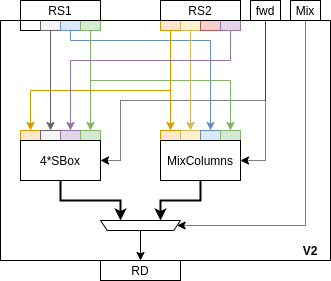
\includegraphics[width={0.5\textwidth}]{diagrams/ise-datapath-v2.png}
\caption{
  A diagramatic description of the functional unit required to support \ISE{2}.
}
\label{fig:v2:fu}
\end{figure}

% =============================================================================

\clearpage
\section{\ISE{3}:       additional technical detail}
\label{sec:pseudo:v3}
% =============================================================================

\vspace*{\fill}

\begin{figure}[!h]
\begin{lstlisting}[language=pseudo,style=block]
saes.v3.encs  rd, rs1, rs2, bs : v3.Proc(rd, rs1, rs2, bs, fwd=1, mix=0)
saes.v3.encsm rd, rs1, rs2, bs : v3.Proc(rd, rs1, rs2, bs, fwd=1, mix=1)
saes.v3.decs  rd, rs1, rs2, bs : v3.Proc(rd, rs1, rs2, bs, fwd=0, mix=0)
saes.v3.decsm rd, rs1, rs2, bs : v3.Proc(rd, rs1, rs2, bs, fwd=0, mix=1)
\end{lstlisting}
\caption{
  Instruction mnemonics, and their mapping onto pseudo-code functions, for \ISE{3}.
}
\label{fig:v3:mnemonics}
\end{figure}

\begin{figure}[!h]
\begin{lstlisting}[language=pseudo,style=block]
v3.Proc(rd, rs1, rs2, bs, fwd, mix):
  x     = AESSBox[rs2.8[bs]] if fwd else AESInvSBox[rs2.8[bs]]
  if   mix and  fwd: t1.32 = {GFMUL(x, 3),      x    ,      x   ,GFMUL(x, 2)}
  elif mix and !fwd: t1.32 = {GFMUL(x,11),GFMUL(x,13),GFMUL(x,9),GFMUL(x,14)}
  else             : t1.32 = {0, 0, 0, x}
  rd.32 = ROTL32(t1.32, 8*bs) ^ rs1
\end{lstlisting}
\caption{
  Instruction pseudo-code functions for \ISE{3}.
}
\label{fig:v3:pseudo}
\end{figure}

\begin{figure}[!h]
\begin{lstlisting}[language=pseudo,style=block]
lw              a0, 16(RK)      // Load Round Key
lw              a1, 20(RK)
lw              a2, 24(RK)
lw              a3, 28(RK)      // t0,t1,t2,t3 contains current round state.
saes.v3.encsm   a0, a0, t0, 0   // Next state for column 0.
saes.v3.encsm   a0, a0, t1, 1   // Current column 0 in t0.
saes.v3.encsm   a0, a0, t2, 2   // Next column 0 accumulates in a0
saes.v3.encsm   a0, a0, t3, 3
saes.v3.encsm   a1, a1, t1, 0   // Next state for column 1.
saes.v3.encsm   a1, a1, t2, 1
saes.v3.encsm   a1, a1, t3, 2
saes.v3.encsm   a1, a1, t0, 3
saes.v3.encsm   a2, a2, t2, 0   // Next state for column 2.
saes.v3.encsm   a2, a2, t3, 1
saes.v3.encsm   a2, a2, t0, 2
saes.v3.encsm   a2, a2, t1, 3
saes.v3.encsm   a3, a3, t3, 0   // Next state for column 3.
saes.v3.encsm   a3, a3, t0, 1
saes.v3.encsm   a3, a3, t1, 2
saes.v3.encsm   a3, a3, t2, 3   // a0,a1,a2,a3 contains new round state
\end{lstlisting}
\caption{
  An AES encryption round implemented using \ISE{3}.
}
\label{fig:v3:round}
\end{figure}

\vspace*{\fill}

% -----------------------------------------------------------------------------

\newpage

\vspace*{\fill}

\begin{figure}[!h]
\centering
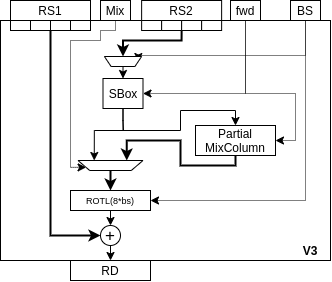
\includegraphics[width={0.5\textwidth}]{diagrams/ise-datapath-v3.png}
\caption{
  A diagrammatic description of the functional unit required to support \ISE{3}.
}
\label{fig:v3:fu}
\end{figure}

\vspace*{\fill}

% =============================================================================

\clearpage
\section{\ISE{4}:       additional technical detail}
\label{sec:pseudo:v4}

%
% V4
% ------------------------------------------------------------

\begin{figure}[h]
\begin{subfigure}{\textwidth}
\begin{lstlisting}[language=pseudo,style=block]
saes.v4.ks1       rd rs1 rcon : v4.ks1(rd, rs1, rcon)
saes.v4.ks2       rd rs1 rs2  : v4.ks2(rd, rs1, rs2 )
saes.v4.imix      rd rs1      : v4.InvMix(rd, rs1)
saes.v4.encsm     rd rs1 rs2  : v4.Enc(rd, rs1, rs2, mix=1)
saes.v4.encs      rd rs1 rs2  : v4.Enc(rd, rs1, rs2, mix=0)
saes.v4.decsm     rd rs1 rs2  : v4.Dec(rd, rs1, rs2, mix=1)
saes.v4.decs      rd rs1 rs2  : v4.Dec(rd, rs1, rs2, mix=0)
\end{lstlisting}
\caption{
\ISE{4} mnemonics and mappings onto pseudo-code functions.
}
\label{fig:mnemonics:v4}
\end{subfigure}
\begin{subfigure}{\textwidth}
\begin{lstlisting}[language=pseudo,style=block]
v4.ks1(rd, rs1, enc_rcon):     // KeySchedule: SubBytes, Rotate, Round Const
    temp.32   = rs1.32[1]
    rcon      = 0x0
    if(enc_rcon != 0xA):
        temp.32 = ROTR32(temp.32, 8)
        rcon    = RoundConstants.8[enc_rcon]
    temp.8[i] = AESSBox[temp.8[i]]  for i=0..3
    temp.8[0] = temp.8[0] ^ rcon
    rd.64     = {temp.32, temp.32}

v4.ks2(rd, rs1, rs2):           // KeySchedule: XOR
    rd.32[0]  = rs1.32[1] ^ rs2.32[0]
    rd.32[1]  = rs1.32[1] ^ rs2.32[0] ^ rs2.32[1]

v4.Enc(rd, rs1, rs2, mix): // SubBytes, ShiftRows, MixColumns
    t1.128    = ShiftRows({rs2, rs1})
    t2.64     = t1.64[0]
    t3.8[i]   = AESSBox[t2.8[i]] for i=0..7
    rd.32[i]  = AESMixColumn(t3.32[i]) if mix else t3.32[i] for i=0..1

v4.Dec(rd, rs1, rs2, mix, hi): // InvSubBytes, InvShiftRows, InvMixColumns
    t1.128    = InvShiftRows(rs2 || rs1)
    t2.64     = t1.64[0]
    t3.8[i]   = AESInvSBox[t2.8[i]] for i=0..7
    rd.32[i]  = AESInvMixColumn(t3.32[i]) if mix else t3.32[i] for i=0..1

v4.InvMix(rd, rs1):             // Inverse MixColumns
    rd.32[i]  = AESInvMixColumn(rs1.32[i]) for i=0..1
\end{lstlisting}
\caption{
    \ISE{4} instruction pseudo-code.
}
\label{fig:pseudo:v4}
\end{subfigure}
\begin{subfigure}{\textwidth}
\begin{lstlisting}[language=pseudo,style=block]
ld              a0, 0(a4)  // Load round key as double words.
ld              a1, 8(a4)
xor             t0, t0, a0 // Add round key for 2 columns at a time.
xor             t1, t1, a1
aes.v5.encsm    t2, t0, t1 // Next round state: columns 0, 1
aes.v5.encsm    t3, t1, t0 // columns 2, 3 - Note swapped rs1/rs2
\end{lstlisting}
\caption{
A single AES encryption round, implemented using \ISE{4}.
}
\label{fig:round:v4}
\end{subfigure}
\caption{
    Mnemonics, pseudo code mappings and example encryption
    round function for \ISE{4}.
}
\end{figure}

\clearpage
\section{\ISE{5}:       additional technical detail}
\label{sec:pseudo:v5}

%
% V5
% ------------------------------------------------------------


\begin{figure}[h]
\begin{subfigure}{\textwidth}
\begin{lstlisting}[language=pseudo,style=block]
saes.v5.esrsub.lo rd, rs1, rs2 : rd = v5.SrSub(rs1, rs2, fwd=1, hi=0)
saes.v5.esrsub.hi rd, rs1, rs2 : rd = v5.SrSub(rs1, rs2, fwd=1, hi=1)
saes.v5.dsrsub.lo rd, rs1, rs2 : rd = v5.SrSub(rs1, rs2, fwd=0, hi=0)
saes.v5.dsrsub.hi rd, rs1, rs2 : rd = v5.SrSub(rs1, rs2, fwd=0, hi=1)
saes.v5.emix      rd, rs1, rs2 : rd = v5.Mix(rs1, rs2, fwd=1)
saes.v5.dmix      rd, rs1, rs2 : rd = v5.Mix(rs1, rs2, fwd=0)
saes.v5.sub       rd, rs1      : rd = SubBytes(rs1.8[i])         for i=0..3
\end{lstlisting}
\caption{
\ISE{5} mnemonics and mappings onto pseudo-code functions.
}
\label{fig:mnemonics:v5}
\end{subfigure}
\begin{subfigure}{\textwidth}
\begin{lstlisting}[language=pseudo,style=block]
v5.SrSub(rd, rs1, rs2, fwd, hi):
  if(fwd):
    if hi: tmp.32 = {rs1.8[3], rs2.8[0], rs2.8[1], rs2.8[2]}
    else : tmp.32 = {rs2.8[3], rs1.8[1], rs1.8[0], rs1.8[2]}
    tmp.8[i]      =    AESSBox[tmp.8[i]] for i=0..3
  else:
    if hi: tmp.32 = {rs2.8[3], rs2.8[0], rs1.8[1], rs2.8[2]}
    else : tmp.32 = {rs1.8[3], rs2.8[1], rs1.8[0], rs1.8[2]}
    tmp.8[i]      = InvAESSBox[tmp.8[i]] for i=0..3
  if(hi): rd.32 = {tmp.8[2],tmp.8[3],tmp.8[0],tmp.8[1]}
  else  : rd.32 = {tmp.8[1],tmp.8[3],tmp.8[0],tmp.8[2]}

v5.mix(rd, rs1, rs2, fwd):
  col0.32 = {rs1.8[2], rs1.8[3], rs2.8[2], rs2.8[3]}
  col1.32 = {rs1.8[0], rs1.8[1], rs2.8[0], rs2.8[1]}
  n0.8    = AESMixColumn(       col0   ) if fwd else AESInvMixColumn(       col0   )
  n1.8    = AESMixColumn(ROTL32(col0,8)) if fwd else AESInvMixColumn(ROTL32(col0,8))
  n2.8    = AESMixColumn(       col1   ) if fwd else AESInvMixColumn(       col1   )
  n3.8    = AESMixColumn(ROTL32(col1,8)) if fwd else AESInvMixColumn(ROTL32(col1,8))
  rd.32 = {n2, n3, n0, n1}
\end{lstlisting}
\caption{
    \ISE{5} instruction pseudo-code.
}
\label{fig:pseudo:v5}
\end{subfigure}
\begin{subfigure}{\textwidth}
\begin{lstlisting}[language=pseudo,style=block]
lw                a0,  0(a4)   // Load Round Key
lw                a1,  4(a4)
lw                a2,  8(a4)
lw                a3, 12(a4)
xor               t0, t0, a0   // Add Round Key
xor               t1, t1, a1
xor               t2, t2, a2
xor               t3, t3, a3
saes.v5.esrsub.lo a0, t0, t1   // Quad 0: SubBytes / ShiftRows
saes.v5.esrsub.lo a1, t1, t0   // Quad 1
saes.v5.esrsub.hi a2, t2, t3   // Quad 2
saes.v5.esrsub.hi a3, t3, t2   // Quad 3
saes.v5.emix      t0, a0, a2   // Quad 0: ShiftRows / MixColumns
saes.v5.emix      t1, a1, a3   // Quad 1
saes.v5.emix      t2, a2, a0   // Quad 2
saes.v5.emix      t3, a3, a1   // Quad 3
\end{lstlisting}
\caption{
A single AES encryption round, implemented using \ISE{1}.
}
\label{fig:round:v5}
\end{subfigure}
\caption{
    Mnemonics, pseudo code mappings and example encryption
    round function for \ISE{5}.
}
\end{figure}


\clearpage
\section{\mbox{\CORE{2}} core: additional technical detail}
\label{sec:core:2}
% =============================================================================

\vspace*{\fill}

\begin{figure}[!h]
\centering
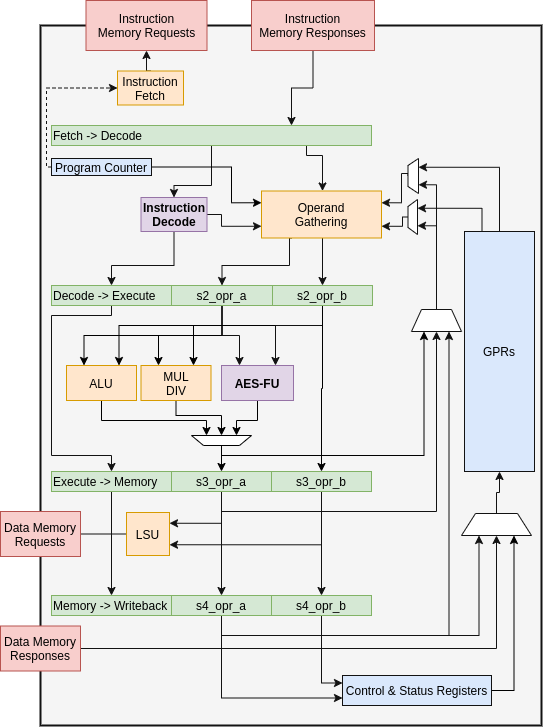
\includegraphics[scale={0.45},angle={90}]{diagrams/scarv-cpu-uarch.png}
\caption{
  \CORE{2} core: vanilla  micro-architecture.
}
\label{fig:core:2:normal}
\end{figure}

% NOTE: Commented out as SCA section not likely to be included in final version.
%\begin{figure}[!h]
%\centering
%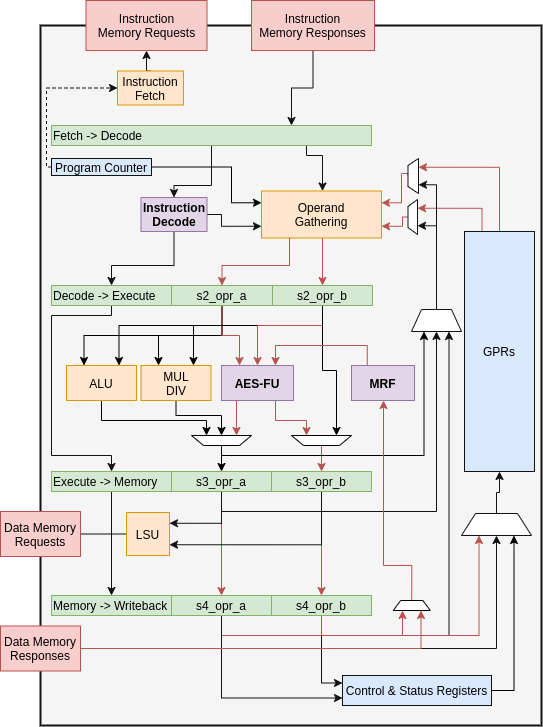
\includegraphics[scale=0.45,angle=90]{diagrams/scarv-cpu-uarch-sca.png}
%\caption{
%  \CORE{2} core: hardened micro-architecture, 
%  extending \ISE{3} for improved security against side-channel attack.
%  Connections coloured red are security-critical, in the sense they relate to masks.
%}
%\label{fig:core:2:secure}
%\end{figure}

\vspace*{\fill}

% =============================================================================

\clearpage
\section{\mbox{\CORE{1}} core: additional technical detail}
\label{sec:core:1}
% =============================================================================

\begin{figure}[!h]
\begin{lstlisting}[style={block},language={scala}]
class AESVanilla32 extends Config (
  new freechips.rocketchip.subsystem.WithNoMMIOPort ++
  new freechips.rocketchip.subsystem.WithNoSlavePort ++
  new freechips.rocketchip.subsystem.WithInclusiveCache ++
  new freechips.rocketchip.subsystem.WithRV32 ++
  new freechips.rocketchip.subsystem.WithNExtTopInterrupts(0) ++
  new freechips.rocketchip.subsystem.WithNBigCores(1) ++
  new freechips.rocketchip.subsystem.WithoutFPU ++
  new freechips.rocketchip.system.BaseConfig
)
\end{lstlisting}
\caption{$32$-bit \CORE{1} core configuration.}
\label{fig:rocket:32}
\end{figure}

\begin{figure}[!h]
\begin{lstlisting}[style={block},language={scala}]
class AESVanilla64 extends Config(
  new freechips.rocketchip.subsystem.WithNoMMIOPort ++
  new freechips.rocketchip.subsystem.WithNoSlavePort ++
  new freechips.rocketchip.subsystem.WithInclusiveCache ++
  new freechips.rocketchip.subsystem.WithNExtTopInterrupts(0) ++
  new freechips.rocketchip.subsystem.WithNBigCores(1) ++
  new freechips.rocketchip.subsystem.WithoutFPU ++
  new freechips.rocketchip.system.BaseConfig
)
\end{lstlisting}
\caption{$64$-bit \CORE{1} core configuration.}
\label{fig:rocket:64}
\end{figure}


% =============================================================================


\clearpage
\section{Additional algorithms}
\label{sec:alg}
% =============================================================================

\begin{algorithm}
\KwData  {A  cipher key             $k$,
          an initialisation vector $iv$,
          and
          an $n$-block  plaintext   $m$.
}
\KwResult{An $n$-block ciphertext   $c$.
}
\BlankLine
\KwFn{$\SCOPE{\ID{AES-CBC}}{\ALG{Enc}}( k, iv, m )$}{
    $c_0 \ASN \SCOPE{\ID{AES}}{\ALG{Enc}}( k, m_0   \XOR iv       )$ \;
  \For{$i = 0$ {\bf upto} $n-1$}{
    $c_i \ASN \SCOPE{\ID{AES}}{\ALG{Enc}}( k, m_i   \XOR  c_{i-1} )$ \;
  }
  \KwRet{$c$} \;
}
\caption{AES-CBC~\cite[Section 6.2]{NIST:sp.800.38a} encryption.}
\label{alg:cbc:enc}
\end{algorithm}

\begin{algorithm}
\KwData  {A  cipher key             $k$,
          an initialisation vector $iv$,
          and
          an $n$-block ciphertext   $c$.
}
\KwResult{An $n$-block  plaintext   $m$.
}
\BlankLine
\KwFn{$\SCOPE{\ID{AES-CBC}}{\ALG{Dec}}( k, iv, c )$}{
    $m_0 \ASN \SCOPE{\ID{AES}}{\ALG{Dec}}( k, c_0 ) \XOR iv        $ \;
  \For{$i = 0$ {\bf upto} $n-1$}{
    $m_i \ASN \SCOPE{\ID{AES}}{\ALG{Dec}}( k, c_i ) \XOR  c_{i-1}  $ \;
  }
  \KwRet{$m$} \;
}
\caption{AES-CBC~\cite[Section 6.2]{NIST:sp.800.38a} decryption.}
\label{alg:cbc:dec}
\end{algorithm}

% =============================================================================

\begin{algorithm}
\KwData  {A  cipher key             $k$,
          an initialisation vector $iv$,
          an increment function     $f$,
          and
          an $n$-block  plaintext   $m$.
}
\KwResult{An $n$-block ciphertext   $c$.
}
\BlankLine
\KwFn{$\SCOPE{\ID{AES-CTR}}{\ALG{Enc}}( k, iv, m )$}{
  $t_0 \ASN iv$ \;
  \For{$i = 0$ {\bf upto} $n-1$}{
    $t_{i+1} \ASN f( t_{i} )$ \;
    $c_{i  } \ASN \SCOPE{\ID{AES}}{\ALG{Enc}}( k, t_{i+1} ) \XOR m_{i}$ \;
  }
  \KwRet{$c$} \;
}
\caption{AES-CTR~\cite[Section 6.5]{NIST:sp.800.38a} encryption.}
\label{alg:ctr:enc}
\end{algorithm}

\begin{algorithm}
\KwData  {A  cipher key             $k$,
          an initialisation vector $iv$,
          an increment function     $f$,
          and
          an $n$-block ciphertext   $c$.
}
\KwResult{An $n$-block  plaintext   $m$.
}
\BlankLine
\KwFn{$\SCOPE{\ID{AES-CTR}}{\ALG{Dec}}( k, iv, m )$}{
  $t_0 \ASN iv$ \;
  \For{$i = 0$ {\bf upto} $n-1$}{
    $t_{i+1} \ASN f( t_{i} )$ \;
    $m_{i  } \ASN \SCOPE{\ID{AES}}{\ALG{Enc}}( k, t_{i+1} ) \XOR c_{i}$ \;
  }
  \KwRet{$m$} \;
}
\caption{AES-CTR~\cite[Section 6.5]{NIST:sp.800.38a} decryption.}
\label{alg:ctr:dec}
\end{algorithm}

% =============================================================================

\begin{algorithm}
\KwData  {A  cipher key             $k$,
          an initialisation vector $iv$,
          an increment function     $f$,
          and
          an $n$-block sequence     $x$.
}
\KwResult{An $n$-block sequence     $y$.
}
\BlankLine
\KwFn{$\SCOPE{\ID{GCM}}{\ALG{GCTR}}( k, iv, f, x )$}{
  $t_0 \ASN iv$ \;
  \For{$i = 0$ {\bf upto} $n-1$}{
    $t_{i+1} \ASN f( t_{i} )$ \;
    $y_{i  } \ASN \SCOPE{\ID{AES}}{\ALG{Enc}}( k, t_{i+1} ) \oplus x_i$ \;
  }
  \KwRet{$y$} \;
}
\caption{The GCTR  component of AES-GCM~\cite[Algorithm 3]{NIST:sp.800.38d}.}
\label{alg:gctr}
\end{algorithm}

% -----------------------------------------------------------------------------

\begin{algorithm}
\KwData  {A  hash   key             $h$,
          and
          an $n$-block sequence     $x$.
}
\KwResult{A         tag             $t$.
}
\BlankLine
\KwFn{$\SCOPE{\ID{GCM}}{\ALG{GHASH}}( h, x )$}{
  $t \ASN 0$ \;
  \For{$i = 0$ {\bf upto} $n-1$}{
    $t \ASN ( t \oplus x_{i} ) \otimes h$
  }
  \KwRet{$t$}
}
\caption{The GHASH component of AES-GCM~\cite[Algorithm 2]{NIST:sp.800.38d}.}
\label{alg:ghash}
\end{algorithm}

% -----------------------------------------------------------------------------

\begin{algorithm}
\KwData  {A  cipher key       $k$,
          a   plaintext block $m$,
          a       tweak block $i$,
          and
          a       block index $j$.
}
\KwResult{A  ciphertext block $c$.
}
\BlankLine
\KwFn{$\SCOPE{\ID{XTS-AES}}{\ALG{Enc}}( k, m, i, j )$}{
  parse $k = k_1 \CONS k_2$ \;
  $t  \ASN \SCOPE{\ID{AES}}{\ALG{Enc}}( k_2, i  ) \otimes \alpha^k$ \;
  $m' \ASN m  \oplus t                                            $ \;
  $c' \ASN \SCOPE{\ID{AES}}{\ALG{Enc}}( k_1, m' )                 $ \;
  $c  \ASN c' \oplus t                                            $ \;
  \KwRet{$c$} \;
}
\caption{XTS-AES~\cite{NIST:sp.800.38e} encryption.}
\label{alg:xts:enc}
\end{algorithm}

\begin{algorithm}
\KwData  {A  cipher key       $k$,
          a  ciphertext block $c$,
          a       tweak block $i$,
          and
          a       block index $j$.
}
\KwResult{A   plaintext block $m$.
}
\BlankLine
\KwFn{$\SCOPE{\ID{XTS-AES}}{\ALG{Dec}}( k, c, i, j )$}{
  parse $k = k_1 \CONS k_2$ \;
  $t  \ASN \SCOPE{\ID{AES}}{\ALG{Enc}}( k_2, i  ) \otimes \alpha^k$ \;
  $c' \ASN c  \oplus t                                            $ \;
  $m' \ASN \SCOPE{\ID{AES}}{\ALG{Enc}}( k_1, c' )                 $ \;
  $m  \ASN m' \oplus t                                            $ \;
  \KwRet{$m$} \;
}
\caption{XTS-AES~\cite{NIST:sp.800.38e} decryption.}
\label{alg:xts:dec}
\end{algorithm}

% =============================================================================


% =============================================================================

\end{document}
